%% This template can be used to write a paper for
%% Computer Physics Communications using LaTeX.
%% For authors who want to write a computer program description,
%% an example Program Summary is included that only has to be
%% completed and which will give the correct layout in the
%% preprint and the journal.
%% The `elsarticle' style is used and more information on this style
%% can be found at 
%% http://www.elsevier.com/wps/find/authorsview.authors/elsarticle.
%%
%%
\documentclass[preprint,12pt]{elsarticle}

%% Use the option review to obtain double line spacing
%% \documentclass[preprint,review,12pt]{elsarticle}

%% Use the options 1p,twocolumn; 3p; 3p,twocolumn; 5p; or 5p,twocolumn
%% for a journal layout:
%% \documentclass[final,1p,times]{elsarticle}
%% \documentclass[final,1p,times,twocolumn]{elsarticle}
%% \documentclass[final,3p,times]{elsarticle}
%% \documentclass[final,3p,times,twocolumn]{elsarticle}
%% \documentclass[final,5p,times]{elsarticle}
%% \documentclass[final,5p,times,twocolumn]{elsarticle}

%% if you use PostScript figures in your article
%% use the graphics package for simple commands
%% \usepackage{graphics}
%% or use the graphicx package for more complicated commands
\usepackage{graphicx}
%% or use the epsfig package if you prefer to use the old commands
%% \usepackage{epsfig}

%% The amssymb package provides various useful mathematical symbols
\usepackage{amssymb}
%% The amsthm package provides extended theorem environments
%% \usepackage{amsthm}

%% Additional needed packages.
\usepackage{amsmath}
\usepackage{verbatim}
\usepackage{color}

%% The lineno packages adds line numbers. Start line numbering with
%% \begin{linenumbers}, end it with \end{linenumbers}. Or switch it on
%% for the whole article with \linenumbers after \end{frontmatter}.
%% \usepackage{lineno}

%% natbib.sty is loaded by default. However, natbib options can be
%% provided with \biboptions{...} command. Following options are
%% valid:

%%   round  -  round parentheses are used (default)
%%   square -  square brackets are used   [option]
%%   curly  -  curly braces are used      {option}
%%   angle  -  angle brackets are used    <option>
%%   semicolon  -  multiple citations separated by semi-colon
%%   colon  - same as semicolon, an earlier confusion
%%   comma  -  separated by comma
%%   numbers-  selects numerical citations
%%   super  -  numerical citations as superscripts
%%   sort   -  sorts multiple citations according to order in ref. list
%%   sort&compress   -  like sort, but also compresses numerical citations
%%   compress - compresses without sorting
%%
%% \biboptions{comma,round}

% \biboptions{}

\newcommand{\pdv}[2]{\frac{\partial{#1}}{\partial{#2}}}
\newcommand{\fp}[2]{\pdv{#1}{#2}}
\newcommand{\pdwc}[3]{\left(\fp{#1}{#2}\right)_{#3}}
%\newcommand{\ppdv}[3]{\displaystyle \frac{\partial^2 #1}{\partial #2\partial #3}}
\newcommand{\ppdv}[3]{\frac{\partial^2 #1}{\partial #2\partial #3}}
\newcommand{\oover}[1]{\ensuremath{\frac{1}{#1}}}

\newcommand{\vect}[1]{\boldsymbol{#1}}
\newcommand{\matr}[1]{\mathbf{#1}}
\newcommand{\dI}{\text{d}}
\newcommand{\odv}[2]{\frac{\dI #1}{\dI #2}}
\newcommand{\ddv}[2]{\odv{#1}{#2}}
\newcommand{\christ}[3]{\genfrac{\{}{\}}{0pt}{}{#1}{#2 #3}}
%\newcommand{\christ}[3]{\Gamma^{#1}_{#2 #3}}
%\newcommand{\ddv}[2]{\frac{\Delta #1}{\Delta #2}}
\newcommand{\collpdv}[2]{\pdv{#1}{#2}\Big|_{coll}}
\newcommand{\mfp}{\lambda}
\newcommand{\tmfp}{\tilde{\lambda}}
\newcommand{\mfpe}{\lambda_e}
\newcommand{\mfpei}{\lambda_{ei}}
\newcommand{\Zbar}{\bar{Z}}
\newcommand{\nue}{\nu_{e}}
\newcommand{\nuei}{\nu_{ei}}
\newcommand{\nutot}{\nu_{t}}
\newcommand{\vmag}{v}
\newcommand{\vth}{v_{th}}
\newcommand{\vn}{\vect{n}}
\newcommand{\E}{\vect{E}}
\newcommand{\B}{\vect{B}}
\newcommand{\tE}{\vect{\tilde{E}}}
\newcommand{\tB}{\vect{\tilde{B}}}
\newcommand{\qe}{q_e}
\newcommand{\me}{m_e}
\newcommand{\kB}{k_B}
\newcommand{\crs}{\sigma}
\newcommand{\fM}{f_M}
\newcommand{\fzero}{f_0}
\newcommand{\vfzero}{\vect{f}_0}
\newcommand{\fone}{\vect{f}_1}
\newcommand{\SM}{\vect{S}_M}
\newcommand{\MI}{\matr{I}}
\newcommand{\MA}{\matr{A}}
\newcommand{\intO}{\int_{\Omega}}
\newcommand{\IM}{\boldsymbol{\mathcal{M}}}
\newcommand{\ID}{\boldsymbol{\mathcal{D}}}
\newcommand{\IV}{\boldsymbol{\mathcal{V}}}
\newcommand{\IB}{\boldsymbol{\mathcal{B}}}
\newcommand{\anisomega}{\fone/\fzero}
\newcommand{\acl}{\vect{M}_{\left(\anisomega\right)}}


\newcommand{\figref}[1]{FIG.~\ref{#1}}
\newcommand{\refeq}[1]{(\ref{#1})}
\newcommand{\secref}[1]{Sec.~\ref{#1}}


%% This list environment is used for the references in the
%% Program Summary
%%
\newcounter{bla}
\newenvironment{refnummer}{%
\list{[\arabic{bla}]}%
{\usecounter{bla}%
 \setlength{\itemindent}{0pt}%
 \setlength{\topsep}{0pt}%
 \setlength{\itemsep}{0pt}%
 \setlength{\labelsep}{2pt}%
 \setlength{\listparindent}{0pt}%
 \settowidth{\labelwidth}{[9]}%
 \setlength{\leftmargin}{\labelwidth}%
 \addtolength{\leftmargin}{\labelsep}%
 \setlength{\rightmargin}{0pt}}}
 {\endlist}

\journal{Computer Physics Communications}

\begin{document}

\begin{frontmatter}

%% Title, authors and addresses

%% use the tnoteref command within \title for footnotes;
%% use the tnotetext command for the associated footnote;
%% use the fnref command within \author or \address for footnotes;
%% use the fntext command for the associated footnote;
%% use the corref command within \author for corresponding author footnotes;
%% use the cortext command for the associated footnote;
%% use the ead command for the email address,
%% and the form \ead[url] for the home page:
%%
%% \title{Title\tnoteref{label1}}
%% \tnotetext[label1]{}
%% \author{Name\corref{cor1}\fnref{label2}}
%% \ead{email address}
%% \ead[url]{home page}
%% \fntext[label2]{}
%% \cortext[cor1]{}
%% \address{Address\fnref{label3}}
%% \fntext[label3]{}

\title{C7: An~efficient 7D plasma kinetic code born to~be~coupled with multi-material ALE~hydrodynamics}

%% use optional labels to link authors explicitly to addresses:
%% \author[label1,label2]{<author name>}
%% \address[label1]{<address>}
%% \address[label2]{<address>}

\author[a]{M. Holec\corref{author}}
%\author[a,b]{Second Author}
%\author[b]{Third Author}

\cortext[author] {Corresponding author.\\\textit{E-mail address:} milan.holec@u-bordeaux.fr}
\address[a]{Centre Lasers Intenses et Applications, Universite de Bordeaux-CNRS-CEA, UMR 5107, F-33405 Talence, France}
%\address[b]{Second Address}

\begin{abstract}
%% Text of abstract
A submitted program is expected to be of benefit to other physicists or physical chemists, or be an exemplar of good programming practice, or illustrate new or novel programming techniques which are of importance to some branch of computational physics or physical chemistry.

Acceptable program descriptions can take different forms. The following Long Write-Up structure is a suggested structure but it is not obligatory. Actual structure will depend on the length of the program, the extent to which the algorithms or software have already been described in literature, and the detail provided in the user manual.

Your manuscript and figure sources should be submitted through the Elsevier Editorial System (EES) by using the online submission tool at \\
http://www.ees.elsevier.com/cpc.

In addition to the manuscript you must supply: the program source code; job control scripts, where applicable; a README file giving the names and a brief description of all the files that make up the package and clear instructions on the installation and execution of the program; sample input and output data for at least one comprehensive test run; and, where appropriate, a user manual. These should be sent, via email as a compressed archive file, to the CPC Program Librarian at cpc@qub.ac.uk.

\end{abstract}

\begin{keyword}
%% keywords here, in the form: keyword \sep keyword
keyword1; keyword2; keyword3; etc.

\end{keyword}

\end{frontmatter}

%%
%% Start line numbering here if you want
%%
% \linenumbers

% Computer program descriptions should contain the following
% PROGRAM SUMMARY.

{\bf PROGRAM SUMMARY}
  %Delete as appropriate.

\begin{small}
\noindent
{\em Program Title:}                                          \\
{\em Licensing provisions(please choose one): CC0 1.0/CC By 4.0/MIT/Apache-2.0/BSD 3-clause/BSD 2-clause/GPLv3/GPLv2/LGPL/CC BY NC 3.0/MPL-2.0 }                                   \\
{\em Programming language:}                                   \\

{\em Supplementary material:}                                 \\
  % Fill in if necessary, otherwise leave out.
{\em Journal reference of previous version:}                  \\
  %Only required for a New Version summary, otherwise leave out.
{\em Does the new version supersede the previous version?:}   \\
  %Only required for a New Version summary, otherwise leave out.
{\em Reasons for the new version:}\\
  %Only required for a New Version summary, otherwise leave out.
{\em Summary of revisions:}*\\
  %Only required for a New Version summary, otherwise leave out.

{\em Nature of problem(approx. 50-250 words):}\\
  %Describe the nature of the problem here. \\
{\em Solution method(approx. 50-250 words):}\\
  %Describe the method solution here.
{\em Additional comments including Restrictions and Unusual features (approx. 50-250 words):}\\
  %Provide any additional comments here.
   \\

%\begin{thebibliography}{0}
%\bibitem{1}Reference 1         % This list should only contain those items referenced in the                 
%\bibitem{2}Reference 2         % Program Summary section.   
%\bibitem{3}Reference 3         % Type references in text as [1], [2], etc.
%                               % This list is different from the bibliography at the end of 
%                               % the Long Write-Up.
%\end{thebibliography}
* Items marked with an asterisk are only required for new versions
of programs previously published in the CPC Program Library.\\
\end{small}

\tableofcontents
%% main text
%\section{}
%\label{}
%---------------------------------------------------------------------
%---------------------------------------------------------------------
\section{Introduction to Tensor Calculus}
\subsection{Transformation properties} 
The~representation of a~tensor in the~Cartesian (reference) coordinate
system is in the~case of tensor of first rank
\begin{equation}
  \vect{x} = \bar{x}^1 \vect{e}_1 + \bar{x}^2 \vect{e}_2 + 
  \bar{x}^3 \vect{e}_3 = \bar{x}^i \vect{e}_i ,
  \label{eq:Cart_vector}
\end{equation}
and in the case of tensor of second rank
\begin{eqnarray}
  \vect{u}\vect{v} = \matr{A} &=& 
  \bar{A}^{11} \vect{e}_1\vect{e}_1  + \bar{A}^{12} \vect{e}_1\vect{e}_2 
  + \bar{A}^{13} \vect{e}_1\vect{e}_3 \nonumber\\
  && \bar{A}^{21} \vect{e}_2\vect{e}_1  + \bar{A}^{22} \vect{e}_2\vect{e}_2 
  + \bar{A}^{23} \vect{e}_2\vect{e}_3\nonumber\\
  && \bar{A}^{31} \vect{e}_3\vect{e}_1  + \bar{A}^{32} \vect{e}_3\vect{e}_2 
  + \bar{A}^{33} \vect{e}_3\vect{e}_3 = \bar{A}^{ij}\vect{e}_i\vect{e}_j 
  = \bar{u}^i\vect{e}_i \bar{v}^j\vect{e}_j ,
  \label{eq:Cart_tensor}
\end{eqnarray}  
where \eqref{eq:Cart_vector} defines the~Cartesian coordinates (vector) 
$\bar{x}^i$ of $\vect{x}$  in orthonormal global basis 
$\vect{e}_1 = [1, 0, 0]$, $\vect{e}_2 = [0, 1, 0]$,
$\vect{e}_3 = [0, 0, 1]$, and \eqref{eq:Cart_tensor} shows the~creation of
second rank tensor $\matr{A}$ as a~outer (tensor) product of first rank tensors
$\vect{u}$ and $\vect{v}$, 
and consequently, its coordinates (matrix) $\bar{A}^{ij} = \bar{u}^i \bar{v}^j$.

While introducing a~general curvilinear coordinates
\begin{eqnarray}
  q^i &=& f^i(\bar{x}^1, \bar{x}^2, \bar{x}^3) , \nonumber \\
  \bar{x}^i &=& g^i(q^1, q^2, q^3) , \nonumber \\
  q_i &=& f_i(\bar{x}_1, \bar{x}_2, \bar{x}_3) , \nonumber \\
  \bar{x}_i &=& g_i(q_1, q_2, q_3) , 
  \label{eq:Curvilinear_coordinates} 
\end{eqnarray}
where the~condition on the~transformation Jacobian to be nonzero
\begin{equation}
  J = \bigg| \pdv{\bar{x}^i}{q^j}\bigg| \neq 0
  \label{eq:transformation}
\end{equation}
is sufficient to have a~well defined curvilinear coordinate system.
It is worth mentioning that two types of coordinates are used in definition
\eqref{eq:Curvilinear_coordinates}, i.e. \textit{covariant} $q_i$ and 
\textit{contravariant} $q^i$ in the case of curvilinear coordinates, and
also in the~case of the~Cartesian coordinates, where the~equality 
$\bar{x}^i = \bar{x}_i$  
holds. The~transformation represented by \eqref{eq:transformation} can be
used to act on \textit{covariant} tensor as
\begin{equation}
  A_{\alpha\beta...\mu} = \pdv{\bar{x}^a}{q^\alpha} \pdv{\bar{x}^b}{q^\beta} ...
  \pdv{\bar{x}^m}{q^\mu} \bar{A}_{ab...m} ,
  \label{eq:covariant_tensor_transformation}
\end{equation}
and the~corresponding inverse transformation can be
used to act on \textit{contravariant} tensor as
\begin{equation}
  A^{\alpha\beta...\mu} = \pdv{q^\alpha}{\bar{x}^a} \pdv{q^\beta}{\bar{x}^b} ...
  \pdv{q^\mu}{\bar{x}^m} \bar{A}^{ab...m} ,
  \label{eq:contravariant_tensor_transformation}
\end{equation}
and finally, in the case of a~mixed tensor the~transformation acts as
\begin{equation}
  A^{\alpha\beta...\mu}_{\kappa\lambda...\nu}  = 
  \pdv{q^\alpha}{\bar{x}^a} \pdv{q^\beta}{\bar{x}^b} ...
  \pdv{q^\mu}{\bar{x}^m}~
  \pdv{\bar{x}^k}{q^\kappa} \pdv{\bar{x}^l}{q^\lambda} ...
  \pdv{\bar{x}^n}{q^\nu} 
  \bar{A}^{ab...m}_{kl...n}.
  \label{eq:mixed_tensor_transformation}
\end{equation}
Equation \eqref{eq:mixed_tensor_transformation} represents a~general rule of
transformation of tensor components $\bar{A}^{ab...m}_{kl...n}$ defined in
the~Cartesian coordinates to the~tensor components 
$A^{\alpha\beta...\mu}_{\kappa\lambda...\nu}$ applying in curvilinear 
coordinates. 
Then, tensor $\matr{A}$ treated in \eqref{eq:mixed_tensor_transformation} 
can be expressed as
\begin{multline}
  \matr{A} = A^{\alpha\beta...\mu}_{\kappa\lambda...\nu} 
  \vect{b}_\alpha\vect{b}_\beta...\vect{b}_\mu
  \vect{b}^{\kappa}\vect{b}^{\lambda}...\vect{b}^{\nu}
  = \bar{A}^{ab...m}_{kl...n}\vect{e}_a\vect{e}_b...\vect{e}_m
  \vect{e}^{k}\vect{e}^{l}...\vect{e}^{n}\\ 
  = \bar{A}^{ab...m...kl...n}\vect{e}_a\vect{e}_b...\vect{e}_m
  \vect{e}_{k}\vect{e}_{l}...\vect{e}_{n}, 
  \label{eq:tensor_representation}
\end{multline}
where $\vect{b}_\alpha$ and $\vect{b}^{\kappa}$ are 
\textit{covariant} and \textit{contravariant} bases in curvilinear coordinates. 
The~last equality in \eqref{eq:tensor_representation} applies only to 
the~global Cartesian basis, because the~\textit{covariant} and 
\textit{contravariant} tensor components and also
the~bases vectors are identical. 
The~\textit{contravariant} basis vectors 
are defined as locally normal to the isosurface created by other coordinates as
\begin{equation}
  \vect{b}^i = \nabla q^i ,
  \label{eq:contravariant_bases}
\end{equation}
and the~\textit{covariant} basis vectors are defined as locally tangent to 
their associated coordinate path-line given by radius vector $\vect{r}$ as
\begin{equation}
  \vect{b}_i = \pdv{\vect{r}}{q^i} ,
  \label{eq:covariant_bases}
\end{equation}
and the~following important equality holds
\begin{equation}
  \vect{b}_i\cdot\vect{b}^j = \delta_i^j ,
  \label{eq:basis_vectors_alignement}
\end{equation}
which stresses the~property, that covariant and contravariant bases vectors
are always aligned in direction.

The~line element can be described in the~Cartesian coordinates as
\begin{equation}
  \dI s^2 = \dI\vect{r}\cdot\dI\vect{r} = 
  (\dI \bar{x}^i \vect{e}_i)\cdot(\dI \bar{x}^j \vect{e}_j) = 
  \vect{e}_i\cdot\vect{e}_j \dI \bar{x}^i \dI \bar{x}^j 
  = \dI \bar{x}^i \dI \bar{x}^i ,
  \label{eq:line_element_Cartesian}
\end{equation}
where the~last equality is due to the~orthonormal Cartesian basis.
The~same line element can be described in the~curvilinear coordinates as
\begin{equation}
  \dI s^2 = \dI\vect{r}\cdot\dI\vect{r} = 
  (\dI q^i \vect{b}_i)\cdot(\dI q^j \vect{b}_j) = 
  \vect{b}_i\cdot\vect{b}_j \dI q^i \dI q^j ,
  \label{eq:line_element_curvilinear}
\end{equation}
More importantly, one can use \eqref{eq:line_element_Cartesian},
\eqref{eq:contravariant_tensor_transformation}, and 
\eqref{eq:line_element_Cartesian} to write
\begin{equation}
  \dI s^2 = \dI \bar{x}^k \dI \bar{x}^k = 
  \pdv{\bar{x}^k}{q^i} \dI q^{i} \pdv{\bar{x}^k}{q^j} \dI q^{j} 
  = \vect{b}_i\cdot\vect{b}_j \dI q^i \dI q^j 
  = g_{ij} \dI q^i \dI q^j ,
  \label{eq:metric_tensor}
\end{equation}
which provides a~fundamental definition of the~metric tensor
\begin{equation}
  g_{ij} = \pdv{\bar{x}^k}{q^i}\pdv{\bar{x}^k}{q^j} 
  = \vect{b}_i\cdot\vect{b}_j .
  \label{eq:metric_tensor_explicit}
\end{equation}
Similarly to \eqref{eq:line_element_curvilinear}
one can find the~definition of contravariant metric tensor
\begin{equation}
  \dI s^2 = \dI\vect{r}\cdot\dI\vect{r} = 
  (\dI q_i \vect{b}^i)\cdot(\dI q_j \vect{b}^j) = 
  \vect{b}^i\cdot\vect{b}^j \dI q_i \dI q_j 
  = g^{ij}\dI q_i \dI q_j ,
  \label{eq:contravariant_metric_tensor}
\end{equation}
It is quite easy to show 
based on \eqref{eq:basis_vectors_alignement}, 
\eqref{eq:metric_tensor_explicit} and \eqref{eq:contravariant_metric_tensor}
that
\begin{equation}
  g_{ij} g^{jk} = \delta_i^k ,
  \label{eq:contravariant_metric_tensor_explicit}
\end{equation}
which represents a~practical way to express the~contravariant metric tensor 
explicitly.

One of the~most useful operations with the~metric tensors is converting 
\textit{contravariant} to \textit{covariant} components and vice versa, i.e.
\begin{equation}
  g_{ij} T^{kj}_{..ab} = T^k_{.iab},\quad g^{ij} T^k_{.iab} = T^{kj}_{..ab} .
  \label{eq:contravariant2covariant}
\end{equation}

\subsection{Tensor operations} 
General tensors obey simple algebraic rules. Thus if 
$\matr{B} = \alpha \matr{A}$ then 
$B^{ab...m}_{kl...n} = \alpha A^{ab...m}_{kl...n}$ and also if
$\matr{C} = \matr{A}\pm\matr{B}$, 
$C^{ab...m}_{kl...n} = A^{ab...m}_{kl...n} \pm B^{ab...m}_{kl...n}$.
Similarly $\matr{A} + \matr{B} = \matr{B} + \matr{A}$ and
$\matr{A} + (\matr{B} + \matr{C}) = (\matr{A} + \matr{B}) + \matr{C}$.

The~meaning of the~\textit{null tensor} $\matr{0}$, i.e. a~tensor whose 
components are all zero in some coordinate system, 
is of a~particular importance,
because it represents a~physical quantity, which is zero in every coordinate
system, as can be seen from  \eqref{eq:mixed_tensor_transformation}.
Consequently, any tensor equation $\matr{A} = \matr{B}$, or component-wise
$A^{ab...m}_{kl...n} = B^{ab...m}_{kl...n}$, is valid in any coordinate system,
because $\matr{A} - \matr{B} = \matr{0}$, and for any two coordinate systems
$\bar{x}^i$ and $q^i$ holds
\begin{equation} 
  \pdv{q^\alpha}{\bar{x}^a} \pdv{q^\beta}{\bar{x}^b} ...
  \pdv{q^\mu}{\bar{x}^m}~
  \pdv{\bar{x}^k}{q^\kappa} \pdv{\bar{x}^l}{q^\lambda} ...
  \pdv{\bar{x}^n}{q^\nu} 
  (\bar{A}^{ab...m}_{kl...n} - \bar{B}^{ab...m}_{kl...n})
  = A^{\alpha\beta...\mu}_{\kappa\lambda...\nu} 
  - B^{\alpha\beta...\mu}_{\kappa\lambda...\nu} = 0 .
  \label{eq:tensor_equation}
\end{equation}

A~special case of a~tensor operation is the~general formula of the~scalar 
product of two vectors, which can be written based
on \eqref{eq:basis_vectors_alignement} and \eqref{eq:contravariant2covariant} as
\begin{equation}
  \vect{u}\cdot\vect{v} = (u^i \vect{b}_i)\cdot(v_j \vect{b}^j) 
  = \vect{b}_i\cdot\vect{b}^j u^i v_j = u^j v_j = g^{ij} u_i v_j = 
  g_{ij} u^i v^j = u_j v^j .
  \label{eq:general_scalar_product}
\end{equation} 
It is worth noting, that even though neither 
\textit{contravariant} nor \textit{covariant} components are in general
real physical representation (have different units), the~product of 
contra- with co-variant components provides physically correct units.

The~general form of the~cross product 
based on the~\textit{Levi-Civita tensor} is given by
\begin{equation}
  \vect{u}\times\vect{v} = \vect{c} = c^i\vect{b}_i = 
  \varepsilon^{ijk}\vect{b}_i\vect{b}_j\vect{b}_k 
  \cdot u_n\vect{b}^n \cdot v_m\vect{b}^m 
  = \varepsilon^{ijk}\vect{b}_i u_j v_k ,
  \nonumber 
\end{equation}
and further can be written the~covariant and contravariant components as
\begin{eqnarray}
  c_i &=& g^{1/2}e_{ijk}u^j v^k = g^{1/2}(u_j v_k - u_k v_j) ,
  \label{eq:general_covariant_cross_product}\\
  c^i &=& g^{-1/2}e^{ijk}u_j v_k = \frac{u_j v_k - u_k v_j}{g^{1/2}} ,
  \label{eq:general_contravariant_cross_product}
\end{eqnarray}
where the~\textit{cyclic permutation} 
(i.e. $i\rightarrow j \rightarrow k \rightarrow i$) is applied 
and the~scaling $\varepsilon^{ijk} = g^{-1/2}e^{ijk}$ and
$\varepsilon_{ijk} = g^{1/2}e_{ijk}$ with respect to curvilinear coordinates
has been used. 

Any tensor of rank two $T^{ij}$ can be uniquely decomposed into a~symmetric 
part and an~antisymmetric part as $\matr{T} = \matr{S} + \matr{A}$, 
which are defined as
\begin{equation}
  S^{ij} = \frac{1}{2}(T^{ij} + T^{ji}),~
  A^{ij} = \frac{1}{2}(T^{ij} - T^{ji}) .
  \label{eq:matrix_decomposition}
\end{equation}

\subsection{Covariant differentiation}
In \cite{Mihalas_Mihalas-Foundations_of_Radiation_Hydrodynamics} a~very 
important result (A3.70) is obtained
\begin{equation}
  \frac{\partial^2\bar{x}^\lambda}{\partial q^i\partial q^j} = 
  \pdv{\bar{x}^\lambda}{q^k}\christ{k}{i}{j} -
  \pdv{\bar{x}^\alpha}{q^i}\pdv{\bar{x}^\beta}{q^j}
  \christ{\lambda}{\alpha}{\beta} ,
  \label{eq:Christ_result}
\end{equation}
where $\christ{i}{j}{k}$ is the~Christoffel symbol of second kind.

If we differentiate the~\textit{covariant} vector
\begin{equation}
  u_i = \pdv{\bar{x}^\alpha}{q^i} \bar{u}_\alpha ,
  \nonumber
\end{equation}
we obtain
\begin{equation}
  u_{i,j} = \pdv{u_i}{q^j} = 
  \pdv{\bar{x}^\alpha}{q^i}\pdv{\bar{x}^\beta}{q^j}
  \pdv{\bar{u}_\alpha}{\bar{x}^\beta} 
  + \frac{\partial^2\bar{x}^\alpha}{\partial q^i\partial q^j} 
  \bar{u}_\alpha 
  = \bar{x}^\alpha_{,i}\bar{x}^\beta_{,j}
  \bar{u}_{\alpha,\beta} 
  + \bar{x}^\alpha_{,ij} 
  \bar{u}_\alpha ,
\end{equation}
which does not represent a~tensor equation, because the~differentiation
in bar coordinate system $\bar{u}_{\alpha,\beta}$ does not transform 
properly to $u_{i,j}$ in curvilinear coordinate system. However, when
multiplying \eqref{eq:Christ_result} by a~vector component in bar space,
we obtain
\begin{equation}
  \pdv{u_i}{q^j} = 
  \pdv{\bar{x}^\alpha}{q^i}\pdv{\bar{x}^\beta}{q^j}
  \pdv{\bar{u}_\alpha}{\bar{x}^\beta} 
  + \pdv{\bar{x}^\lambda}{q^k}\christ{k}{i}{j}\bar{u}_\lambda
  - \pdv{\bar{x}^\alpha}{q^i}\pdv{\bar{x}^\beta}{q^j}
  \christ{\lambda}{\alpha}{\beta}\bar{u}_\lambda .
  \nonumber
\end{equation}
This can be finally rewritten as
\begin{equation}
  u_{i;j} = \pdv{u_i}{q^j} 
  - \christ{k}{i}{j} u_k
  = \pdv{\bar{x}^\alpha}{q^i}\pdv{\bar{x}^\beta}{q^j}
  \left(\pdv{\bar{u}_\alpha}{\bar{x}^\beta} 
  - \christ{\lambda}{\alpha}{\beta}\bar{u}_\lambda\right) ,
  \label{eq:vector_covariant_diff}
\end{equation}
which represents definition of \textit{covariant differentiation} of vector
$u_{i;j}$, which apparently obeys the~tensor transformation.

The~\textit{covariant differentiation} of a~general tensor reads
\begin{multline}
  A^{ab...m}_{kl...n;j} = \pdv{A^{ab...m}_{kl...n}}{q^j} 
  + \christ{a}{j}{d}A^{db...m}_{kl...n}
  + \christ{b}{j}{d}A^{ad...m}_{kl...n} + ...
  + \christ{m}{j}{d}A^{ab...d}_{kl...n} \\
  - \christ{d}{j}{k}A^{ab...m}_{dl...n}
  - \christ{d}{j}{l}A^{ab...m}_{kd...n} - ...
  - \christ{d}{j}{n}A^{ab...m}_{kl...d} ,
\end{multline} 
where the~notation above means 
the~$^{ab...m}_{kl...n}$ component of the~differentiation of tensor 
$\matr{A}$ along the~covariant basis vector $\vect{b}_j$.

For the~sake of applicability, some \textit{covariant differentiation}
explicit formulas of tensors of various ranks are presented
\begin{eqnarray}
  f_{;j} &=& (\nabla f)_j = f_{,j} , \label{eq:cd_scalar}\\
  u^a_{;j} &=& (\nabla u^a)_j = u^a_{,j} + \christ{a}{j}{k} u^k , 
  \label{eq:cd_contravector} \\
  u_{a;j} &=& (\nabla u_a)_j = u_{a,j} - \christ{k}{j}{a} u_k , 
  \label{eq:cd_covector} \\
  A^{ab}_{;j} &=& (\nabla A^{ab})_j = A^{ab}_{,j} + \christ{a}{j}{k} A^{kb} 
  + \christ{b}{j}{k} A^{ak} , 
  \label{eq:cd_contratensor} \\
  A_{ab;j} &=& (\nabla A_{ab})_j = A_{ab,j} - \christ{k}{j}{a} A_{kb} 
  - \christ{k}{j}{b} A_{ak} ,
  \label{eq:cd_cotensor} \\
  A^a_{b;j} &=& (\nabla A^a_{b})_j = A_{ab,j} + \christ{a}{j}{k} A^k_b
  - \christ{k}{j}{b} A^a_k ,
  \label{eq:cd_mixedtensor}
\end{eqnarray} 
where $f$ is a~scalar function, $\vect{u}$ is a~vector field, and
$\matr{A}$ is a~second rank tensor field.

\subsection{General form of Gradient, Divergence, Laplace, and Curl}
Covariant generalization of operations with the~\textit{del operator} $\nabla$
can in most instances be obtained simply by replacing the~partial derivatives
in the~Cartesian coordinate system with covariant derivatives.

Then, the~gradient operator acting on a~general tensor $\nabla \matr{A}$ can
be expressed component-wise as
\begin{equation}
  \nabla A^{ab...m}_{kl...n} = (\nabla A^{ab...m}_{kl...n})_j\vect{b}^j 
  = A^{ab...m}_{kl...n;j}\vect{b}^j .
  \label{eq:general_grad}
\end{equation}
Consequently, the~divergence operation on a~vector field reads
\begin{equation}
  \nabla\cdot\vect{v} = \nabla_i\vect{b}^i\cdot v^j\vect{b}_j 
  = (\vect{b}^i\cdot\vect{b}_j) \nabla_i v^j = \delta^i_j \nabla_i v^j
  = \nabla_i v^i = v^i_{;i} = v^i_{,i} + \christ{i}{i}{j}v^j ,
  \nonumber
\end{equation}
where the~right hand side can be further simplified and the~general form
of divergence reads
\begin{equation}
  \nabla\cdot\vect{v} = v^i_{;i} = \frac{(g^{1/2}v^i)_{,i}}{g^{1/2}} ,
  \label{eq:general_divvec}
\end{equation}
where $g$ is the~determinant of the~metric tensor $\matr{g}$.

The~tensor contraction due to the~divergence operation on its second component
reads
\begin{equation}
  T^{ij}_{;j} = \frac{(g^{1/2}S^{ij})_{,j}}{g^{1/2}} + \christ{i}{j}{k}S^{jk} 
  + \frac{(g^{1/2}A^{ij})_{,j}}{g^{1/2}} ,
  \label{eq:general_divtens}
\end{equation}
where the~decomposition \eqref{eq:matrix_decomposition} has been used.

The~Laplace operator in curvilinear coordinate system acts as
\begin{equation}
  \nabla\cdot\nabla f = \nabla_j\vect{b}^j\cdot g^{ik}f_{,i}\vect{b}_k = 
  \delta^j_k \nabla_j (g^{ik}f_{,i}) = \nabla_j (g^{ij}f_{,i}) 
  = (g^{ij}f_{,i})_{;j} , 
  \nonumber
\end{equation}
where the~contravariant representation $f^{,k} = g^{ik}f_{,i}$ of gradient
of scalar function has been used.
Then the~general form of Laplace operator can be written as
\begin{equation}
  \nabla\cdot\nabla f = \frac{(g^{1/2}g^{ij}f_{,i})_{,j}}{g^{1/2}} .
  \label{eq:general_Laplace}
\end{equation}

The~contravariant generalization of the~curl of vector can be obtained while
using the~Levi-Civita tensor and covariant derivative
\begin{equation}
  (\nabla\times\vect{u})^i = g^{-1/2}e^{ijk} u_{k;j} 
  = g^{-1/2} (u_{k;j} - u_{j;k}) ,
  \nonumber
\end{equation} 
however, since the~Christoffel symbols of second kind are symmetric in lower 
indices, the~general form of curl can be written as 
\begin{equation}
  (\nabla\times\vect{u})^i = g^{-1/2} (u_{k,j} - u_{j,k}) ,
  \label{eq:general_curlvec}
\end{equation} 
where $(i,j,k)$ are distinct and are a~cyclic permutation of (1,2,3).

\subsection{Spherical coordinates}
Spherical coordinates, also called spherical polar coordinates 
(Walton 1967, Arfken 1985), are a system of curvilinear coordinates with 
local orthogonal basis that are natural for describing positions on a~sphere 
or spheroid. Define $\theta$ to be the azimuthal angle in the $xy$-plane from 
the~x-axis with $0<\theta<2\pi$, $\phi$ to be the polar angle from 
the~positive z-axis with $0<\phi<\pi$, and $r$ to be distance (radius) from 
a~point to the~origin. This is the convention commonly used in mathematics. 

Based on the~curvilinear coordinates transformation 
\eqref{eq:Curvilinear_coordinates}
\begin{equation}
  r = \sqrt{x^2 + y^2 + z^2} ,~ 
  \phi = \cos^{-1} \left( \frac{z}{\sqrt{x^2 + y^2 + z^2}} \right),~
  \theta = \tan^{-1}\left( \frac{y}{x} \right) ,
  \label{eq:spher_curvilinear_transformation}
\end{equation}
and its Cartesian inverse
\begin{equation}
  x = r \cos(\theta)\sin(\phi) ,~ 
  %\nonumber\\
  y = r \sin(\theta)\sin(\phi) ,~ 
  %\nonumber\\
  z = r \cos(\phi),
  \label{eq:spher_Cartesian_transformation}
\end{equation}
we can write the~spherical curvilinear transformation
\begin{equation}
  \matr{T}_{s} = \begin{bmatrix}
        \pdv{x}{r} & \pdv{x}{\phi} & \pdv{x}{\theta} \\
        \pdv{y}{r} & \pdv{y}{\phi} & \pdv{y}{\theta} \\
        \pdv{z}{r} & \pdv{z}{\phi} & \pdv{z}{\theta} 
	  \end{bmatrix}
  = \begin{bmatrix}
  \cos(\theta)\sin(\phi) & r\cos(\theta)\cos(\phi) & -r\sin(\theta)\sin(\phi) \\
  \sin(\theta)\sin(\phi) & r\sin(\theta)\cos(\phi) & r\cos(\theta)\sin(\phi) \\
  \cos(\phi) & -r\sin(\phi) & 0  
  \end{bmatrix} ,
  \label{eq:spher_transformation}
\end{equation}
which is well defined \eqref{eq:transformation}
\begin{equation}
  J = |\matr{T}_{s}| = r^2\sin(\phi) = g_s^{1/2}.
  \label{eq:spher_J}
\end{equation}
Then according to \eqref{eq:metric_tensor_explicit} we can express the~metric
tensor (diagonal for orthogonal basis) as
\begin{equation}
  \matr{g}_s = \begin{bmatrix}
                 g_{rr} & 0 & 0 \\
			     0 & g_{\phi\phi} & 0 \\
			     0 & 0 & g_{\theta\theta}
			   \end{bmatrix}
             = \begin{bmatrix}
                 1 & 0 & 0 \\
			     0 & r^2 & 0 \\
			     0 & 0 & r^2\sin^2(\phi)
			   \end{bmatrix} .
  \label{eq:spher_metric_tensor}		   
\end{equation}
From \eqref{eq:basis_vectors_alignement} it is obvious, 
that in general contravariant basis vectors are aligned with covariant basis 
vectors, and are inverse in magnitude.
It can be directly observed, that the~covariant basis vectors are orthogonal
from \eqref{eq:metric_tensor_explicit} and explicit formulation of 
the~metric tensor \eqref{eq:spher_metric_tensor}, which further provides
the~information about the~basis vectors length
\begin{equation}
  |\vect{b}_r| = 1,~ |\vect{b}_\phi| = r,~ |\vect{b}_\theta| = r\sin(\phi), 
  \nonumber
\end{equation} 
and from \eqref{eq:basis_vectors_alignement} one can directly write
\begin{equation}
  |\vect{b}^r| = 1,~ |\vect{b}^\phi| = \frac{1}{r},~ 
  |\vect{b}^\theta| = \frac{1}{r\sin(\phi)}.
  \nonumber
\end{equation}
It makes sense to define the~scaling
\begin{equation}
  h_r = 1,~ h_\phi = r,~ h_\theta = r\sin(\phi), 
  \label{eq:spher_scaling}
\end{equation} 
which comes to be handy when defining the~relation between 
\textit{physical}, \textit{covariant}, and \textit{contravariant} components as
\begin{equation}
  \vect{u} = u^i \vect{b}_i = u_i \vect{b}^i = \sum_i u^i h_i \vect{e}_i
  = \sum_i \frac{u_i}{h_i} \vect{e}_i = u(i) \vect{e}_i,
  \label{eq:spher_components}
\end{equation}
where a~unique basis vectors $\vect{e}_i$ have been used, because they are 
identical for both covariant and contravariant bases, and they are also used
as the~basis for physical components $u(i)$.
The~explicit relations between physical, covariant, and contravariant components
of vector in spherical coordinates are
\begin{eqnarray}
  u(r) &=& u^r = u_r , \nonumber\\ 
  u(\phi) &=& u^\phi r = \frac{u_\phi}{r} , \nonumber\\
   u(\theta) &=& u^\theta r\sin(\phi) = \frac{u_\theta}{r\sin(\phi)} ,
  \label{eq:spher_physical_components}
\end{eqnarray}

The~scalar product of two vectors $\vect{u}$ and $\vect{v}$ expressed 
in physical components $u(i), v(j)$ in spherical coordinates can be expressed 
based on \eqref{eq:general_scalar_product} as
\begin{equation}
  \vect{u}\cdot\vect{v} = u_i v^i = u(r)v(r) + u(\phi)v(\phi) 
  + u(\theta)v(\theta) .
  \label{eq:spher_scalar_product}
\end{equation}
The~cross product of two vectors $\vect{u}$ and $\vect{v}$ expressed 
in physical components $u(i), v(j)$ in spherical coordinates can be expressed 
based on \eqref{eq:general_contravariant_cross_product} 
and \eqref{eq:spher_components} as
\begin{multline}
  \vect{u}\times\vect{v} = \vect{c} = c^i \vect{b}_i = 
  c^r \vect{b}_r + c^\phi \vect{b}_\phi
  + c^\theta \vect{b}_\theta \\
  = \frac{1}{r^2\sin(\phi)}\left[
  (u_\phi v_\theta - u_\theta v_\phi) \vect{b}_r 
  +  (u_\theta v_r - u_r v_\theta) \vect{b}_\phi
  +  (u_r v_\phi - u_\phi v_r)\vect{b}_\theta
  \right] \\
  = \frac{1}{r^2\sin(\phi)}\left[
  (u_\phi v_\theta - u_\theta v_\phi) \vect{e}_r 
  +  (u_\theta v_r - u_r v_\theta) r\vect{e}_\phi
  +  (u_r v_\phi - u_\phi v_r)r\sin(\phi)\vect{e}_\theta
  \right] \\
 %= \frac{1}{r^2\sin(\phi)}\left[
 % (r u(\phi) r\sin(\phi)v(\theta) - r\sin(\phi)u(\theta) r v(\phi)) \vect{e}_r 
 % +  (r\sin(\phi)u(\theta) v(r) - u(r) r\sin(\phi)v(\theta)) \vect{e}_\phi
 % +  (u(r) r v(\phi) - r u(\phi) v(r))\vect{e}_\theta
 % \right] \\ 
 = [u(\phi) v(\theta) - u(\theta) v(\phi)] \vect{e}_r
 + [u(\theta) v(r) - u(r) v(\theta)] \vect{e}_\phi
 + [u(r) v(\phi) - u(\phi) v(r)]\vect{e}_\theta .
 \label{eq:spher_cross_product}
\end{multline}
%$c^i = \frac{u_j v_k - u_k v_j}{g^{1/2}}$

The~gradient of a~scalar function $f$ in spherical coordinates based on 
\eqref{eq:general_grad} reads
\begin{equation}
  \nabla f = f_{,i}\vect{b}^i = \pdv{f}{r}\vect{e}_r 
  + \frac{1}{r}\pdv{f}{\phi}\vect{e}_\phi
  + \frac{1}{r\sin(\phi)}\pdv{f}{\theta}\vect{e}_{\theta} .
  \label{eq:spher_gradf}
\end{equation}
The~divergence of a~vector field $\vect{v}$ in spherical coordinates based on
\eqref{eq:general_divvec} reads
\begin{multline}
  \nabla\cdot\vect{u} = v^i_{;i} = 
  \frac{(r^2\sin(\phi)v^i)_{,i}}{r^2\sin(\phi)}
  = \pdv{v^r}{r} + \pdv{v^\phi}{\phi} + \pdv{v^\theta}{\theta} 
  + \frac{2v^r}{r} + \cot(\phi) v^\phi \\
  = \pdv{v(r)}{r} + \pdv{(v(\phi)/r)}{\phi} 
  + \pdv{(v(\theta)/r\sin(\phi))}{\theta} 
  + \frac{2 v(r)}{r} + \cot(\phi) v(\phi)/r \\
  = \frac{1}{r^2}\pdv{(r^2v(r))}{r} 
  + \frac{1}{r\sin(\phi)}\pdv{(\sin(\phi)v(\phi))}{\phi} 
  + \frac{1}{r\sin(\phi)}\pdv{v(\theta)}{\theta} .
  \label{eq:spher_gradf}
\end{multline}

In the~case of Laplacian operator, we first need to find the~contravariant 
representation of gradient, i.e.
\begin{equation}
  \nabla f = f^{,j}\vect{b}_j = g^{ij} f_{,i}\vect{b}_j 
  = \pdv{f}{r}\vect{b}_r + \frac{1}{r^2}\pdv{f}{\phi}\vect{b}_\phi
  + \frac{1}{r^2\sin^2(\phi)}\pdv{f}{\theta}\vect{b}_{\theta} ,
  \nonumber
\end{equation}
then, the~Laplace of a~scalar $f$ in spherical coordinates based on
\eqref{eq:general_Laplace} reads
\begin{multline}
  \nabla\cdot\nabla f = (f^{,i})_{;i} = 
  \frac{(r^2\sin(\phi)f^{,i})_{,i}}{r^2\sin(\phi)} \\
  = \frac{1}{r^2\sin(\phi)}\left( \pdv{}{r}\left(r^2\sin(\phi)f_{,r} \right) 
  + \pdv{}{\phi}\left(\sin(\phi) f_{,\phi} \right)
  + \pdv{}{\theta}\left(\frac{f_{,\theta}}{\sin(\phi)}\right) \right) \\
  = \frac{1}{r^2}\pdv{}{r}\left(r^2\pdv{f}{r} \right) 
  + \frac{1}{r^2\sin(\phi)} \pdv{}{\phi}\left(\sin(\phi) \pdv{f}{\phi}\right)
  + \frac{1}{r^2\sin^2(\phi)} \frac{\partial^2 f}{\partial\theta^2} .
  \label{eq:spher_Laplacef}
\end{multline}

The~physical components of curl applied on a~vector field $\vect{v}$ 
in spherical coordinates based on \eqref{eq:general_curlvec}, 
i.e. $(\nabla\times\vect{u})^i = g^{-1/2} (u_{k,j} - u_{j,k})$, are
\begin{eqnarray}
  (\nabla\times\vect{v})(r) &=& (\nabla\times\vect{v})^r 
  = \frac{v_{\theta,\phi} - v_{\phi,\theta}}{r^2\sin(\phi)} 
  = \frac{1}{r\sin(\phi)}
  \left[\pdv{(\sin(\phi)v(\theta))}{\phi} - \pdv{v(\phi)}{\theta} \right] , 
  \nonumber \\
  (\nabla\times\vect{v})(\phi) &=& (\nabla\times\vect{v})^\phi r 
  = \frac{v_{r,\theta} - v_{\theta,r}}{r^2\sin(\phi)} r  
  = \frac{1}{r}
  \left[\frac{1}{\sin(\phi)}\pdv{v(r)}{\theta} 
  - \pdv{(r v(\theta))}{r} \right] , 
  \nonumber \\
  (\nabla\times\vect{v})(\theta) &=& (\nabla\times\vect{v})^\theta r\sin(\phi) 
  = \frac{v_{\phi,r} - v_{r, \phi}}{r^2\sin(\phi)} r\sin(\phi) 
  = \frac{1}{r}
  \left[\pdv{(r v(\phi))}{r} 
  - \pdv{v(r)}{\phi} \right] , \nonumber
\end{eqnarray}
where one should be aware, that the~coordinates follow the~order 
$(r, \phi, \theta)$.
Then, the~curl applied on a~vector field $\vect{v}$ in spherical coordinates 
based on \eqref{eq:general_curlvec} reads
\begin{multline}
  \nabla\times\vect{v} = 
  \frac{1}{r\sin(\phi)}
  \left[\pdv{(\sin(\phi)v(\theta))}{\phi} - \pdv{v(\phi)}{\theta} \right] 
  \vect{e}_r\\
  + \frac{1}{r}
  \left[\frac{1}{\sin(\phi)}\pdv{v(r)}{\theta} 
  - \pdv{(r v(\theta))}{r} \right]
  \vect{e}_\phi
  + \frac{1}{r}
  \left[\pdv{(r v(\phi))}{r} 
  - \pdv{v(r)}{\phi} \right] 
  \vect{e}_\theta .
  \label{eq:spher_curlvec}
\end{multline}

\subsection{Cylindrical coordinates}
Cylindrical coordinates are a~generalization of two-dimensional polar 
coordinates to three dimensions by superposing a~height ($z$) axis. 
Unfortunately, there are a~number of different notations used for 
the~other two coordinates. Either  $r$ or $\rho$ is used to refer to 
the~radial coordinate and either $\phi$ or $\theta$ to the~azimuthal 
coordinates. Arfken (1985), for instance, uses $(\rho,\phi,z)$, 
while Beyer (1987) uses $(r,\theta,z)$. 
In this work, the~notation $(r,\theta,z)$ is used.

Based on the~curvilinear coordinates transformation 
\eqref{eq:Curvilinear_coordinates}
\begin{equation}
  r = \sqrt{x^2 + z^2} ,~ 
  %\nonumber\\
  \theta = \tan^{-1}\left( \frac{y}{x} \right) ,~ 
  %\nonumber\\
  z = z,
  \label{eq:cyl_curvilinear_transformation}
\end{equation}
and its Cartesian inverse
\begin{equation}
  x = r \cos(\theta) ,~ 
  %\nonumber\\
  y = r \sin(\theta) ,~ 
  %\nonumber\\
  z = z,
  \label{eq:cyl_Cartesian_transformation}
\end{equation}
we can write the~cylindrical curvilinear transformation
\begin{equation}
  \matr{T}_{s} = \begin{bmatrix}
        \pdv{x}{r} & \pdv{x}{\theta} & \pdv{x}{z} \\
        \pdv{y}{r} & \pdv{y}{\theta} & \pdv{y}{z} \\
        \pdv{z}{r} & \pdv{z}{\theta} & \pdv{z}{z} 
	  \end{bmatrix}
  = \begin{bmatrix}
  \cos(\theta) & -r\sin(\theta) & 0 \\
  \sin(\theta) & r\cos(\theta) & 0 \\
  0 & 0 & 1
  \end{bmatrix} ,
  \label{eq:cyl_transformation}
\end{equation}
which is well defined \eqref{eq:transformation}
\begin{equation}
  J = |\matr{T}_{s}| = r = g_c^{1/2}.
  \label{eq:cyl_J}
\end{equation}
Then according to \eqref{eq:metric_tensor_explicit} we can express the~metric
tensor (diagonal for orthogonal basis) as
\begin{equation}
  \matr{g}_s = \begin{bmatrix}
                 g_{rr} & 0 & 0 \\
			     0 & g_{\theta\theta} & 0 \\
			     0 & 0 & g_{zz}
			   \end{bmatrix}
             = \begin{bmatrix}
                 1 & 0 & 0 \\
			     0 & r^2 & 0 \\
			     0 & 0 & 1
			   \end{bmatrix} .
  \label{eq:cyl_metric_tensor}		   
\end{equation}
From \eqref{eq:basis_vectors_alignement} it is obvious, 
that in general contravariant basis vectors are aligned with covariant basis 
vectors, and are inverse in magnitude.
It can be directly observed, that the~covariant basis vectors are orthogonal
from \eqref{eq:metric_tensor_explicit} and explicit formulation of 
the~metric tensor \eqref{eq:cyl_metric_tensor}, which further provides
the~information about the~basis vectors length
\begin{equation}
  |\vect{b}_r| = 1,~ |\vect{b}_\theta| = r,~ |\vect{b}_z| = 1,
  \nonumber
\end{equation} 
and from \eqref{eq:basis_vectors_alignement} one can directly write
\begin{equation}
  |\vect{b}^r| = 1,~ |\vect{b}^\theta| = \frac{1}{r},~ 
  |\vect{b}^z| = 1.
  \nonumber
\end{equation}
It makes sense to define the~scaling
\begin{equation}
  h_r = 1,~ h_\theta = r,~ h_z = 1,
  \label{eq:cyl_scaling}
\end{equation} 
which comes to be handy when defining the~relation between 
\textit{physical}, \textit{covariant}, and \textit{contravariant} components as
\begin{equation}
  \vect{u} = u^i \vect{b}_i = u_i \vect{b}^i = \sum_i u^i h_i \vect{e}_i
  = \sum_i \frac{u_i}{h_i} \vect{e}_i = u(i) \vect{e}_i,
  \label{eq:cyl_components}
\end{equation}
where a~unique basis vectors $\vect{e}_i$ have been used, because they are 
identical for both covariant and contravariant bases, and they are also used
as the~basis for physical components $u(i)$.
The~explicit relations between physical, covariant, and contravariant components
of vector in cylindrical coordinates are
\begin{eqnarray}
  u(r) &=& u^r = u_r , \nonumber\\
  u(\theta) &=& u^\theta r = \frac{u_\theta}{r} , 
  \nonumber\\
  u(z) &=& u^z = u_z , 
  \label{eq:cyl_physical_components}
\end{eqnarray}

The~scalar product of two vectors $\vect{u}$ and $\vect{v}$ expressed 
in physical components $u(i), v(j)$ in cylindrical coordinates can be expressed 
based on \eqref{eq:general_scalar_product} as
\begin{equation}
  \vect{u}\cdot\vect{v} = u_i v^i = u(r)v(r) + u(\theta)v(\theta) 
  + u(z)v(z) .
  \label{eq:cyl_scalar_product}
\end{equation}
The~cross product of two vectors $\vect{u}$ and $\vect{v}$ expressed 
in physical components $u(i), v(j)$ in cylindrical coordinates can be expressed 
based on \eqref{eq:general_contravariant_cross_product} 
and \eqref{eq:cyl_components} as
\begin{multline}
  \vect{u}\times\vect{v} = \vect{c} = c^r \vect{b}_r 
  + c^\theta \vect{b}_\theta + c^z \vect{b}_z \\
  = \frac{1}{r}\left[
  (u_\theta v_z - u_z v_\theta) \vect{b}_r 
  +  (u_z v_r - u_r v_z) \vect{b}_\theta
  +  (u_r v_\theta - u_\theta v_r)\vect{b}_z
  \right] \\
  = \frac{1}{r}\left[
  (u_\theta v_z - u_z v_\theta) \vect{e}_r 
  +  (u_z v_r - u_r v_z) r\vect{e}_\theta
  +  (u_r v_\theta - u_\theta v_r)\vect{e}_z
  \right] \\
 %= \frac{1}{r}\left[
 % (r u(\theta) v(z) - u(z) r v(\theta)) \vect{e}_r 
 % +  (u(z) v(r) - u(r) v(z)) \vect{e}_\theta
 % +  (u(r) r v(\theta) - r u(\theta) v(r))\vect{e}_z
 % \right] \\ 
 = [u(\theta) v(z) - u(z) v(\theta)] \vect{e}_r
 + [u(z) v(r) - u(r) v(z)] \vect{e}_\theta 
 + [u(r) v(\theta) - u(\theta) v(r)]\vect{e}_z .
 \label{eq:cyl_cross_product}
\end{multline}
%$c^i =  \frac{u_j v_k - u_k v_j}{g^{1/2}}$

The~gradient of a~scalar function $f$ in cylindrical coordinates based on 
\eqref{eq:general_grad} reads
\begin{equation}
  \nabla f = f_{,i}\vect{b}^i = \pdv{f}{r}\vect{e}_r 
  + \frac{1}{r}\pdv{f}{\theta}\vect{e}_{\theta} 
  + \pdv{f}{z}\vect{e}_z .
  \label{eq:cyl_gradf}
\end{equation}
The~divergence of a~vector field $\vect{v}$ in cylindrical coordinates based on
\eqref{eq:general_divvec}
\begin{multline}
  \nabla\cdot\vect{u} = v^i_{;i} = 
  \frac{(r v^i)_{,i}}{r}
  = \pdv{v^r}{r} + \pdv{v^\theta}{\theta} 
  + \pdv{v^z}{z} + \frac{v^r}{r} \\
  = \frac{1}{r}\pdv{(r v(r))}{r} + \frac{1}{r}\pdv{v(\theta)}{\theta} 
  + \pdv{v(z)}{z} .
  \label{eq:cyl_gradf}
\end{multline}

In the~case of Laplacian operator, we first need to find the~contravariant 
representation of gradient, i.e.
\begin{equation}
  \nabla f = f^{,j}\vect{b}_j = g^{ij} f_{,i}\vect{b}_j 
  = \pdv{f}{r}\vect{b}_r 
  + \frac{1}{r^2}\pdv{f}{\theta}\vect{b}_{\theta}
  + \pdv{f}{z}\vect{b}_z ,
  \nonumber
\end{equation}
then, the~Laplace of a~scalar $f$ in cylindrical coordinates based on
\eqref{eq:general_Laplace} reads
\begin{multline}
  \nabla\cdot\nabla f = (f^{,i})_{;i} = 
  \frac{(r f^{,i})_{,i}}{r} 
  = \frac{1}{r}\left( \pdv{}{r}\left(r f_{,r} \right) 
  + \pdv{}{\theta}\left(\frac{f_{,\theta}}{r}\right)
  + \pdv{}{z} f_{,z} \right) \\
  = \frac{1}{r}\pdv{}{r}\left(r\pdv{f}{r} \right) 
  + \frac{1}{r^2} \frac{\partial^2 f}{\partial\theta^2}
  + \frac{\partial^2 f}{\partial z^2}
  =  \frac{\partial^2 f}{\partial r^2}
  + \frac{1}{r^2} \frac{\partial^2 f}{\partial\theta^2}
  + \frac{\partial^2 f}{\partial z^2} + \frac{1}{r}\pdv{f}{r} .
  \label{eq:cyl_Laplacef}
\end{multline}

The~physical components of curl applied on a~vector field $\vect{v}$ 
in cylindrical coordinates based on \eqref{eq:general_curlvec}, 
i.e. $(\nabla\times\vect{u})^i = g^{-1/2} (u_{k,j} - u_{j,k})$, are
\begin{eqnarray}
  (\nabla\times\vect{v})(r) &=& (\nabla\times\vect{v})^r 
  = \frac{v_{z, \theta} - v_{\theta, z}}{r} 
  = \frac{1}{r} \pdv{v(z))}{\theta} - \pdv{v(\theta)}{z} , 
  \nonumber \\
  (\nabla\times\vect{v})(\theta) &=& (\nabla\times\vect{v})^\theta r 
  = \frac{v_{r,z} - v_{z,r}}{r} r  
  = \pdv{v(r)}{z} - \pdv{v(z)}{r} , 
  \nonumber \\
  (\nabla\times\vect{v})(z) &=& (\nabla\times\vect{v})^z 
  = \frac{v_{\theta,r} - v_{r, \theta}}{r} 
  = \frac{1}{r}
  \left[\pdv{(r v(\theta))}{r} 
  - \pdv{v(r)}{\theta} \right] , \nonumber
\end{eqnarray}
where one should be aware, that the~coordinates follow the~order 
$(r, \theta, z)$.
Then, the~curl applied on a~vector field $\vect{v}$ in cylindrical coordinates 
based on \eqref{eq:general_curlvec} reads
\begin{equation}
  \nabla\times\vect{v} = 
  \left[ \frac{1}{r} \pdv{v(z))}{\theta} - \pdv{v(\theta)}{z} \right] 
  \vect{e}_r
  + \left[ \pdv{v(r)}{z} - \pdv{v(z)}{r} \right] \vect{e}_\theta
  + \frac{1}{r} \left[\pdv{(r v(\theta))}{r} - \pdv{v(r)}{\theta} \right] 
  \vect{e}_z .
  \label{eq:cyl_curlvec}
\end{equation}

\section{Diffusive regime}
The~equilibrium (maximized entropy) distribution
\begin{equation}
  \fM = \frac{\rho}{\vth^3 \left( 2 \pi \right)^{3/2}} 
  \exp\left(- \frac{\vmag^2}{2 \vth^2} \right) ,
  \label{eq:MBdistribution}
\end{equation}
where $\vth = \sqrt{\kB T/\me}$.
\begin{eqnarray}
  \pdv{\fM}{\vmag} &=& -\frac{\vmag}{\vth^2}\fM ,
  \nonumber \\
  \pdv{\fM}{\rho} &=& \frac{1}{\rho}\fM ,
  \nonumber \\
  \pdv{\fM}{T} &=& \left( \frac{\vmag^2}{2 \vth^2} - \frac{3}{2}\right)
  \frac{1}{T}\fM. 
  \nonumber
\end{eqnarray}

\subsection{Lorentz approximation}\label{sec:Lorentz_cop}
\begin{equation}
  \vect{v}\cdot\nabla_{\vect{x}} f 
  + \frac{\qe}{\me}\left(\E + \frac{1}{c}\vect{v}\times\B\right)\cdot
  \nabla_{\vect{v}}f = 
  C_e(f)
  + \frac{\rho\sigma_{ei}}{2}\nabla_{\vect{v}}\cdot
  \left[\frac{1}{\vmag}
  \left(\matr{\delta} - \frac{\vect{v}\vect{v}}{\vmag^2} \right)\cdot
  \nabla_{\vect{v}} f\right] ,
  \label{eq:Lorentz}
\end{equation}

\begin{equation}
  C_{ei}(f, f_i) = 
  \frac{\rho\sigma}{2}\nabla_{\vect{v}}\cdot
  \left[\frac{1}{\vmag}
  \left(\matr{\delta} - \frac{\vect{v}\vect{v}}{\vmag^2} \right)\cdot
  \nabla_{\vect{v}} f\right] ,
  \label{eq:ei_collision_operator}
\end{equation}

\begin{equation}
  \vect{v} = \vmag\vn = \vmag\vect{b}^\vmag = \vmag\vect{b}_\vmag ,
  \label{eq:v}
\end{equation}

\begin{equation}
  \matr{\delta} = \delta^i_j \vect{b}_i \vect{b}^j ,
  \label{eq:delta}
\end{equation}

\begin{equation}
  \nabla_{\vect{v}} f = f^{,j}\vect{b}_j = g^{ij} f_{,i}\vect{b}_j 
  = \pdv{f}{\vmag}\vect{b}_\vmag + \frac{1}{\vmag^2}\pdv{f}{\phi}\vect{b}_\phi
  + \frac{1}{\vmag^2\sin^2(\phi)}\pdv{f}{\theta}\vect{b}_{\theta} 
  = u^j\vect{b}_j = \vect{u} ,
  \nonumber
\end{equation}

\begin{equation}
  \matr{\delta}\cdot\vect{u} = 
  \delta^i_j\vect{b}_i\vect{b}^j\cdot u^k\vect{b}_k =  
  \delta^i_j\vect{b}_i \delta^j_k u^k = \delta^i_k\vect{b}_i u^k 
  = u^k \vect{b}_k = \vect{u} ,
  \nonumber
\end{equation}

\begin{eqnarray}
  \left(\matr{\delta} - \frac{\vect{v}\vect{v}}{\vmag^2} \right)
  \cdot\nabla_{\vect{v}} f &=& 
  \pdv{f}{\vmag}\vect{b}_\vmag + \frac{1}{\vmag^2}\pdv{f}{\phi}\vect{b}_\phi
  + \frac{1}{\vmag^2\sin^2(\phi)}\pdv{f}{\theta}\vect{b}_{\theta} \nonumber \\ 
  &&- \vect{b}_\vmag\vect{b}^\vmag\cdot\left[\pdv{f}{\vmag}\vect{b}_\vmag 
  + \frac{1}{\vmag^2}\pdv{f}{\phi}\vect{b}_\phi
  + \frac{1}{\vmag^2\sin^2(\phi)}\pdv{f}{\theta}\vect{b}_{\theta} \right]
  \nonumber \\
  &=& \pdv{f}{\vmag}\vect{b}_\vmag 
  + \frac{1}{\vmag^2}\pdv{f}{\phi}\vect{b}_\phi
  + \frac{1}{\vmag^2\sin^2(\phi)}\pdv{f}{\theta}\vect{b}_{\theta}  
  - \pdv{f}{\vmag}\vect{b}_\vmag \nonumber \\
  &=& \frac{1}{\vmag^2}\pdv{f}{\phi}\vect{b}_\phi
  + \frac{1}{\vmag^2\sin^2(\phi)}\pdv{f}{\theta}\vect{b}_{\theta} 
  = u^i\vect{b}_i ,
\end{eqnarray}

\begin{eqnarray}
  C_{ei}(f, f_i) &=& \frac{\sigma\rho}{2}\left(\frac{1}{\vmag}u^i\right)_{;i} 
  = \frac{\sigma\rho}{2} \frac{(g^{1/2} \frac{1}{\vmag}u^i)_{,i}}{g^{1/2}}
  = \frac{\sigma\rho}{2} \frac{(\vmag\sin(\phi)u^i)_{,i}}{\vmag^2\sin(\phi)}
  \nonumber\\
  &=& \frac{\sigma\rho}{2} \frac{1}{\vmag^2\sin(\phi)}
  \left[\pdv{}{\phi}\left(\frac{\sin(\phi)}{\vmag}\pdv{f}{\phi}\right)
  + \pdv{}{\theta}\left(\frac{1}{\vmag\sin(\phi)}\pdv{f}{\theta}\right) \right]
  \nonumber\\
  &=& \frac{\sigma\rho}{2\vmag^3} \frac{1}{\sin(\phi)}
  \left[\pdv{}{\phi}\left(\sin(\phi)\pdv{f}{\phi}\right)
  + \frac{1}{\sin(\phi)}\frac{\partial^2f}{\partial\theta^2} \right]
\end{eqnarray}

\begin{equation}
  \odv{f}{\phi} = \pdv{f}{\cos(\phi)}\pdv{\cos{\phi}}{\phi} 
  = - \pdv{f}{\cos(\phi)}\sin(\phi)
\end{equation}

\begin{equation}
  C_{ei}(f, f_i) = \frac{\sigma\rho}{2\vmag^3} 
  \left(\pdv{}{\mu}\left((1 - \mu^2)\pdv{f}{\mu}\right)
  + \frac{1}{\sin^2(\phi)}\frac{\partial^2f}{\partial\theta^2} \right)
\end{equation}
where $\mu = \cos(\phi)$

First, the~electro-magnetic scaling
\begin{equation}
  \tE = \frac{\qe}{\me}\E,~\tB = \frac{\qe}{\me c} \B,
\end{equation}
is defined in order to make the~algebraic operations easier to follow.

\begin{eqnarray}
  \vmag\vn\cdot\nabla f 
  &=& - \left(\tE + \vmag\vn\times\tB\right)\cdot
  \left[ \pdv{f}{\vmag}\vn 
  + \frac{1}{\vmag}\pdv{f}{\phi}\vect{e}_\phi
  + \frac{1}{\vmag\sin(\phi)}\pdv{f}{\theta}\vect{e}_{\theta} \right] 
  \nonumber \\
  &+& C_e(f) 
  + \frac{\nu_{ei}}{2} 
  \left(\pdv{}{\mu}\left((1 - \mu^2)\pdv{f}{\mu}\right)
  + \frac{1}{\sin^2(\phi)}\frac{\partial^2f}{\partial\theta^2} \right) 
  \nonumber \\
  &=& - \Big(
  \left[\left(\tE\cdot\vn\right)\vn 
  + \left(\tE\cdot\vect{e}_\phi\right)\vect{e}_\phi
  + \left(\tE\cdot\vect{e}_\theta\right)\vect{e}_\theta \right] 
  \nonumber \\
  &+& \vmag\vn\times
  \left[\left(\tB\cdot\vn\right)\vn 
  + \left(\tB\cdot\vect{e}_\phi\right)\vect{e}_\phi
  + \left(\tB\cdot\vect{e}_\theta\right)\vect{e}_\theta \right] \Big)\cdot 
  \nonumber \\
  && \left[ \pdv{f}{\vmag}\vn 
  + \frac{1}{\vmag}\pdv{f}{\phi}\vect{e}_\phi
  + \frac{1}{\vmag\sin(\phi)}\pdv{f}{\theta}\vect{e}_{\theta} \right] 
  \nonumber \\
  &+& C_e(f)
  + \frac{\nu_{ei}}{2} 
  \left(\pdv{}{\mu}\left((1 - \mu^2)\pdv{f}{\mu}\right)
  + \frac{1}{\sin^2(\phi)}\frac{\partial^2f}{\partial\theta^2} \right) 
  \nonumber \\ 
  &=& - \Big(
  \left[\tilde{E}(\vmag)\vn 
  + \tilde{E}(\phi)\vect{e}_\phi
  + \tilde{E}(\theta)\vect{e}_\theta \right] 
  + \vmag
  \left[\tilde{B}(\phi)\vect{e}_\theta 
  - \tilde{B}(\theta)\vect{e}_\phi \right] \Big)\cdot 
  \nonumber \\
  && \left[ \pdv{f}{\vmag}\vn 
  + \frac{1}{\vmag}\pdv{f}{\phi}\vect{e}_\phi
  + \frac{1}{\vmag\sin(\phi)}\pdv{f}{\theta}\vect{e}_{\theta} \right] 
  \nonumber \\
  &+& C_e(f)
  + \frac{\nu_{ei}}{2} 
  \left(\pdv{}{\mu}\left((1 - \mu^2)\pdv{f}{\mu}\right)
  + \frac{1}{\sin^2(\phi)}\frac{\partial^2f}{\partial\theta^2} \right)
  \nonumber \\
  &=& - \Bigg(
  \left[ \tilde{E}(\vmag)\pdv{f}{\vmag} 
  + \frac{\tilde{E}(\phi)}{\vmag}\pdv{f}{\phi}
  + \frac{\tilde{E}(\theta)}{\vmag\sin(\phi)}\pdv{f}{\theta} \right]
  \nonumber \\ 
  &+& \vmag
  \left[\frac{\tilde{B}(\phi)}{\vmag\sin(\phi)}\pdv{f}{\theta}
  - \frac{\tilde{B}(\theta)}{\vmag}\pdv{f}{\phi} \right] \Bigg)
  \nonumber \\
  &+& C_e(f) 
  + \frac{\nu_{ei}}{2} 
  \left(\pdv{}{\mu}\left((1 - \mu^2)\pdv{f}{\mu}\right)
  + \frac{1}{\sin^2(\phi)}\frac{\partial^2f}{\partial\theta^2} \right)
  \label{eq:BGK_spherical_definition}
\end{eqnarray}

\begin{multline}
  \vect{v}\cdot\nabla f + \tE\cdot\vn \pdv{f}{\vmag} 
  + \frac{\tE\cdot\vect{e}_\phi 
  - \vmag\tB\cdot\vect{e}_\theta}{\vmag}\pdv{f}{\phi}
  + \frac{\tE\cdot\vect{e}_\theta + \vmag\tB\cdot\vect{e}_\phi}
  {\vmag\sin(\phi)}\pdv{f}{\theta} 
  =\\
  C_e(f) 
  + \frac{\nu_{ei}}{2} 
  \left(\pdv{}{\mu}\left((1 - \mu^2)\pdv{f}{\mu}\right)
  + \frac{1}{\sin^2(\phi)}\frac{\partial^2f}{\partial\theta^2} \right) ,
  \label{eq:Lorentz_spherical}
\end{multline}

\subsubsection{BGK collision operator}\label{sec:BGK_cop}
The~BGK electron transport equation in 6D reads
\begin{multline}
  \vn\cdot\nabla f + \frac{1}{\vmag} \left[ \tE\cdot\vn \pdv{f}{\vmag} 
  + \frac{\tE\cdot\vect{e}_\phi 
  - \vmag\tB\cdot\vect{e}_\theta}{\vmag}\pdv{f}{\phi}
  + \frac{\tE\cdot\vect{e}_\theta + \vmag\tB\cdot\vect{e}_\phi}
  {\vmag\sin(\phi)}\pdv{f}{\theta} \right] 
  =\\
  \frac{\left(\fM - f\right)}{\lambda^e} 
  + \frac{1}{2 \lambda^{ei}} 
  \left(\pdv{}{\mu}\left((1 - \mu^2)\pdv{f}{\mu}\right)
  + \frac{1}{\sin^2(\phi)}\frac{\partial^2f}{\partial\theta^2} \right) ,
  \label{eq:BGK_spherical}
\end{multline}
where $\mu = \cos(\phi)$, $\mfpe$ is the~electron-electron mean free path, and
$\mfpei$ is the~electron-ion mean free path. We also approximate
$\mfpe = \Zbar \mfpei$.

%We can try to find an~approximate solution while using the~first term of
%expansion in $\mfp$, $\cos(\phi)$, $\sin(\phi)$, $\sin(\theta)$, and $\fM$ as
%\begin{equation}
%  f = f^0 + f^1 \mfp\fM\cos(\phi) + f^2 \mfp\fM\sin(\phi)\sin(\theta),
%  \label{eq:f_approximation}
%\end{equation}
\begin{comment} % fM approximation
We can try to find an~approximate solution while using the~first term of
expansion in $\mfpe$, $mu$, and $\fM$ as
\begin{equation}
  \tilde{f}(z, \vmag, \mu) = f^0(z, \vmag) + f^1(\vmag) \mfpei\fM(z, \vmag)\mu .
  \label{eq:f_approximation}
\end{equation}
Clearly, $\pdv{\tilde{f}}{\theta} = 0$, and if $\tB = \tilde{B}_z\vect{e}_z$, 
there is no effect of magnetic field. We also assume, that 
$\nabla f = \pdv{f}{z}\vect{e}_z$ and appropriately 
$\tE = \tilde{E}_z\vect{e}_z$.
From the~orientation of the~Cartesian basis vectors and spherical 
basis vectors, one can find $\tE\cdot\vn = \tilde{E}_z \cos(\phi) = \mu$ and
$\tE\cdot\vect{e}_\phi = -\tilde{E}_z\sin(\phi)$. As a~result, the~analyzed
BGK equation reads
\begin{multline}
  \mu\pdv{}{z}\left( f^0 + f^1 \mfpei\fM\mu \right) 
  + \frac{1}{\vmag} \left[ \tilde{E}_z\mu \pdv{}{\vmag} 
  \left( f^0 + f^1 \mfpei\fM\mu \right) 
  - \frac{\tilde{E}_z\sin(\phi)}{\vmag}\pdv{}{\phi} 
  \left( f^0 + f^1 \mfpei\fM\mu \right)
  \right] 
  =\\
  \frac{\left(\fM - \left( f^0 + f^1 \mfpei\fM\mu \right) \right)}{\mfpe} 
  + \frac{1}{2 \mfpei}\pdv{}{\mu}\left((1 - \mu^2)
  \pdv{}{\mu}\left( f^0 + f^1 \mfpei\fM\mu \right) \right) ,
  \label{eq:BGK_spherical}
\end{multline}

\begin{multline}
  \mu\pdv{f^0}{z} + \mu^2 \pdv{}{z}\left(f^1 \mfpei\fM \right)
  + \frac{\tilde{E}_z}{\vmag} \left[ \mu \pdv{f^0}{\vmag} 
  + \mu^2 \pdv{}{\vmag} \left( f^1 \mfpei\fM \right) 
  + \frac{1 - \mu^2}{\vmag}f^1 \mfpei\fM
  \right] 
  =\\
  \frac{\fM - f^0}{\Zbar\mfpei} - \mu \frac{1}{\Zbar}f^1 \fM
  - \mu
  f^1 \fM ,
  \label{eq:BGK_spherical}
\end{multline}
consequently, we have the~following anisotropy expansion 
$\mu^0, \mu^1, \mu^2, ...$ equations
\begin{eqnarray}
  \frac{\fM - f^0}{\mfpe} &=& \frac{1}{\vmag}f^1 \mfpei\fM , 
  \nonumber \\
  \pdv{f^0}{z} + \frac{\tilde{E}_z}{\vmag}\pdv{f^0}{\vmag} &=& 
  - \frac{1}{\Zbar}f^1 \fM - f^1 \fM , 
  \nonumber \\ 
  \pdv{}{z}\left(f^1 \mfpei\fM \right) 
  + \frac{\tilde{E}_z}{\vmag} \left[\pdv{}{\vmag} \left( f^1 \mfpei\fM \right)
  - \frac{1}{\vmag}f^1 \mfpei\fM \right] &=& 0 , \nonumber
\end{eqnarray}
which lead to the~definitions
\begin{eqnarray}
  f^0 &=& \fM + \frac{1}{\vmag}f^1 \mfpei^2\fM ,
  \label{eq:BGK_f0} \\
  f^1 &=& - \frac{1}{\fM}\frac{\Zbar}{\Zbar+1}
  \left[ \pdv{f^0}{z} + \frac{\tilde{E}_z}{\vmag}\pdv{f^0}{\vmag} \right] 
  \nonumber \\
  &=& - \frac{\Zbar}{\Zbar+1}
  \left[\frac{1}{\rho}\pdv{\rho}{z} + 
  \left( \frac{\vmag^2}{2 \vth^2} - \frac{3}{2}\right)
  \frac{1}{T}\pdv{T}{z} - \frac{\tilde{E}_z}{\vth^2} \right] 
  \nonumber \\
  &=& - \frac{\Zbar}{\Zbar+1}
  \left( \frac{\vmag^2}{2 \vth^2} - \frac{3}{2} - \alpha\right)
  \frac{1}{T}\pdv{T}{z} ,
  \label{eq:BGK_f1}
\end{eqnarray}
\end{comment} % fM approximation
We can try to find an~approximate solution while using the~first term of
expansion in $\mfpe$ and $mu$as
\begin{equation}
  \tilde{f}(z, \vmag, \mu) = f^0(z, \vmag) + f^1(z, \vmag) \mfpei\mu .
  \label{eq:f_approximation}
\end{equation}
Clearly, $\pdv{\tilde{f}}{\theta} = 0$, and if $\tB = \tilde{B}_z\vect{e}_z$, 
there is no effect of magnetic field. We also assume, that 
$\nabla f = \pdv{f}{z}\vect{e}_z$ and appropriately 
$\tE = \tilde{E}_z\vect{e}_z$.
From the~orientation of the~Cartesian basis vectors and spherical 
basis vectors, one can find $\tE\cdot\vn = \tilde{E}_z \cos(\phi) = \mu$ and
$\tE\cdot\vect{e}_\phi = -\tilde{E}_z\sin(\phi)$. As a~result, the~analyzed
BGK equation reads
\begin{multline}
  \mu\pdv{}{z}\left( f^0 + f^1 \mfpei\mu \right) 
  + \frac{1}{\vmag} \left[ \tilde{E}_z\mu \pdv{}{\vmag} 
  \left( f^0 + f^1 \mfpei\mu \right) 
  - \frac{\tilde{E}_z\sin(\phi)}{\vmag}\pdv{}{\phi} 
  \left( f^0 + f^1 \mfpei\mu \right)
  \right] 
  =\\
  \frac{\left(\fM - \left( f^0 + f^1 \mfpei\mu \right) \right)}{\mfpe} 
  + \frac{1}{2 \mfpei}\pdv{}{\mu}\left((1 - \mu^2)
  \pdv{}{\mu}\left( f^0 + f^1 \mfpei\mu \right) \right) ,
  \label{eq:BGK_spherical}
\end{multline}

\begin{multline}
  \mu\pdv{f^0}{z} + \mu^2 \pdv{}{z}\left(f^1 \mfpei \right)
  + \frac{\tilde{E}_z}{\vmag} \left[ \mu \pdv{f^0}{\vmag} 
  + \mu^2 \pdv{}{\vmag} \left( f^1 \mfpei \right) 
  + \frac{1 - \mu^2}{\vmag}f^1 \mfpei
  \right] 
  =\\
  \frac{\fM - f^0}{\Zbar\mfpei} - \mu \frac{1}{\Zbar}f^1
  - \mu f^1 ,
  \label{eq:BGK_spherical}
\end{multline}
consequently, we have the~following anisotropy expansion 
$\mu^0, \mu^1, \mu^2, ...$ equations
\begin{eqnarray}
  \frac{\fM - f^0}{\Zbar\mfpei} &=& \frac{1}{\vmag}f^1 \mfpei , 
  \nonumber \\
  \pdv{f^0}{z} + \frac{\tilde{E}_z}{\vmag}\pdv{f^0}{\vmag} &=& 
  - \frac{1}{\Zbar}f^1 - f^1 , 
  \nonumber \\ 
  \pdv{}{z}\left(f^1 \mfpei \right) 
  + \frac{\tilde{E}_z}{\vmag} \left[\pdv{}{\vmag} \left( f^1 \mfpei \right)
  - \frac{1}{\vmag}f^1 \mfpei \right] &=& 0 , \nonumber
\end{eqnarray}
which lead to the~definitions
\begin{eqnarray}
  f^0 &=& \fM + \frac{1}{\vmag}f^1 \Zbar\mfpei^2 ,
  \label{eq:BGK_f0} \\
  f^1 &=& - \frac{\Zbar}{\Zbar+1}
  \left[ \pdv{f^0}{z} + \frac{\tilde{E}_z}{\vmag}\pdv{f^0}{\vmag} \right] 
  \nonumber \\
  &=& - \frac{\Zbar}{\Zbar+1}
  \left[\frac{1}{\rho}\pdv{\rho}{z} + 
  \left( \frac{\vmag^2}{2 \vth^2} - \frac{3}{2}\right)
  \frac{1}{T}\pdv{T}{z} - \frac{\tilde{E}_z}{\vth^2} \right]\fM 
  %\nonumber \\
  %&=& - \frac{\Zbar}{\Zbar+1}
  %\left( \frac{\vmag^2}{2 \vth^2} - \frac{3}{2} - \alpha\right)
  %\frac{1}{T}\pdv{T}{z}\fM ,
  \label{eq:BGK_f1}
\end{eqnarray}

In order to ensure the~plasma to be quasi-neutral, the~zero-current condition
\begin{equation}
  \vect{j} = \int_0^{\infty}\int_{4\pi} \qe \vmag \vn f 
  \, \dI\vn~\vmag^2~\dI\vmag 
  = \vect{0} ,
  \label{eq:zero_current}
\end{equation}
can be achieved by providing a~consistent electric field in 
\eqref{eq:f_approximation}, i.e.
\begin{equation}
  \tE = \frac{\vth^2~\int_{4\pi} \vn\otimes\vn\cdot \int_0^{\infty} \vmag  
  \fM \frac{\mfp}{\alpha}\left(\frac{\nabla\rho}{\rho} + 
  \left( \frac{\vmag^2}{2 \vth^2} - \frac{3}{2}\right) 
  \frac{\nabla T}{T}\right)
  \vmag^2\, \dI\vmag\, \dI\vn}
  {\int_{4\pi} \vn\otimes\vn\cdot \int_0^{\infty} \vmag  
  \fM \frac{\mfp}{\alpha}\vmag^2\, \dI\vmag\, \dI\vn} ,
\end{equation}
which may be further simplified as
\begin{equation}
  \tE = \frac{\int_0^{\infty} \fM
  \frac{1}{2}\frac{\nabla T}{T}\vmag^9\, \dI\vmag}
  {\int_0^{\infty} \fM \vmag^7\, \dI\vmag} + 
  \vth^2\left(\frac{\nabla\rho}{\rho} - \frac{3}{2}\frac{\nabla T}{T} \right)
  = \vth^2\left(\frac{\nabla\rho}{\rho} + \frac{5}{2}\frac{\nabla T}{T} 
  \right) ,
\end{equation}
where it is worth mentioning, that the~part 
$\fM + \frac{\vmag\mfp}{\alpha} \pdv{f_1}{\vmag}$ of the~distribution
does not contribute to the~current since it is isotropic.
One can write the~quasi-neutral distribution function explicitly 
distinguishing between original part (blue color) and E field correction
(red color) as
\begin{equation}
  f \approx \fM \left(1 - \frac{\mfp}{\alpha}\vn\cdot\left( 
  \textcolor{blue}{
  \frac{\vmag^2}{2 \vth^2} - \frac{3}{2}
  }
  \textcolor{red}{
  - \frac{5}{2}
  }
  \right) \frac{\nabla T}{T} \right) 
  + \frac{\vmag\mfp}{\alpha} \pdv{f_1}{\vmag} .
  \label{eq:f_localized_quasineutral}
\end{equation}
which leads to the~resulting heat flux
\begin{equation}
  \vect{q}_H = \int_{4\pi}\int_0^{\infty} \frac{\me \vmag^2}{2} \vmag \vn f 
  \vmag^2\, \dI\vmag\, \dI\vn = \frac{4\pi}{3}\frac{\me}{2}
  \frac{1}{\alpha \crs\rho}
  \int_0^{\infty} \left( 
  \textcolor{blue}{
  \frac{\vmag^2}{2 \vth^2} - \frac{3}{2}
  }
  \textcolor{red}{
  - \frac{5}{2}
  }
  \right) \vmag^9 \fM\, \dI\vmag \frac{\nabla T}{T} .
  \nonumber
\end{equation} 
Based on the~Gauss integral formula
\begin{equation}
  \int \vmag^{2s+1} \exp\left(-\frac{\vmag^2}{2\vth^2}\right)\, \dI\vmag = 
  \frac{s!~(2 \vth^2)^{s+1}}{2}
  \nonumber 
\end{equation}
and Maxwell-Boltzmann distribution \eqref{eq:MBdistribution} the~heat flux can 
be written as
\begin{equation}
  \vect{q}_H = \frac{4\pi}{3}\frac{\me}{2}\frac{1}{\alpha \crs\rho}
  \frac{\rho}{\vth^3 \left( 2 \pi \right)^{3/2}}
  \frac{4!~2^4 \vth^{10}}{T} \left( 
  \textcolor{blue}{
  5 - \frac{3}{2}
  }
  \textcolor{red}{
  - \frac{5}{2}
  }
  \right) \nabla T 
  = \frac{\me}{\alpha \crs}\frac{128}{\sqrt{2 \pi}}
  \left(\frac{\kB}{\me}\right)^{\frac{7}{2}}T^{\frac{5}{2}} \nabla T .
  \label{eq:Lorentz_flux}
\end{equation} 
In conclusion, equation \eqref{eq:Lorentz_flux} provides nothing else than
the~well known Lorentz approximation heat flux and its nonlinearity $2.5$
in temperature. What is worth mentioning is the~effect of E field 
(quasi-neutrality), which reduces the~flux of about	71.4$\%$ 
(also assuming constant density).


Finally, one can find the~approximate solution
\begin{equation}
  \tilde{f} = \fM - \mfpei\frac{\Zbar}{\Zbar+1}
  \left( \frac{\vmag^2}{2 \vth^2} - \frac{3}{2} - \alpha\right)
  \frac{\vn\cdot\nabla T}{T}\fM .
  \label{eq:BGK_approximate_solution}
\end{equation}


\subsubsection{AWBS collision operator}\label{sec:AWBS_cop}
The~AWBS electron transport equation in 6D reads
\begin{multline}
  \vn\cdot\nabla f + \frac{1}{\vmag} \left[ \tE\cdot\vn \pdv{f}{\vmag} 
  + \frac{\tE\cdot\vect{e}_\phi 
  - \vmag\tB\cdot\vect{e}_\theta}{\vmag}\pdv{f}{\phi}
  + \frac{\tE\cdot\vect{e}_\theta + \vmag\tB\cdot\vect{e}_\phi}
  {\vmag\sin(\phi)}\pdv{f}{\theta} \right] 
  =\\
  \frac{\vmag}{\lambda^e}\pdv{}{\vmag}\left(f - f_M\right) 
  + \frac{1}{2 \lambda^{ei}} 
  \left(\pdv{}{\mu}\left((1 - \mu^2)\pdv{f}{\mu}\right)
  + \frac{1}{\sin^2(\phi)}\frac{\partial^2f}{\partial\theta^2} \right) ,
  \label{eq:AWBS_spherical}
\end{multline}
where $\mu = \cos(\phi)$, $\mfpe$ is the~electron-electron mean free path, and
$\mfpei$ is the~electron-ion mean free path.

We can try to find an~approximate solution while using the~first term of
expansion in $\mfpe$ and $\mu$ as
\begin{equation}
  \tilde{f}(z, \vmag, \mu) = f^0(z, \vmag) + f^1(z, \vmag) \mfpei\mu .
  \label{eq:f_approximation}
\end{equation}
Clearly, $\pdv{\tilde{f}}{\theta} = 0$, and if $\tB = \tilde{B}_z\vect{e}_z$, 
there is no effect of magnetic field. We also assume, that 
$\nabla f = \pdv{f}{z}\vect{e}_z$ and appropriately 
$\tE = \tilde{E}_z\vect{e}_z$.
From the~orientation of the~Cartesian basis vectors and spherical 
basis vectors, one can find $\tE\cdot\vn = \tilde{E}_z \cos(\phi) = \mu$ and
$\tE\cdot\vect{e}_\phi = -\tilde{E}_z\sin(\phi)$. As a~result, the~analyzed
AWBS equation reads
\begin{multline}
  \mu\pdv{}{z}\left( f^0 + f^1 \mfpei\mu \right) 
  + \frac{1}{\vmag} \left[ \tilde{E}_z\mu \pdv{}{\vmag} 
  \left( f^0 + f^1 \mfpei\mu \right) 
  - \frac{\tilde{E}_z\sin(\phi)}{\vmag}\pdv{}{\phi} 
  \left( f^0 + f^1 \mfpei\mu \right)
  \right] 
  =\\
  \frac{\vmag}{\mfpe}\pdv{}{\vmag}
  \left(\left( f^0 + f^1 \mfpei\mu \right) -\fM\right)
  + \frac{1}{2 \mfpei}\pdv{}{\mu}\left((1 - \mu^2)
  \pdv{}{\mu}\left( f^0 + f^1 \mfpei\mu \right) \right) ,
  \label{eq:AWBS_spherical}
\end{multline}

\begin{multline}
  \mu\pdv{f^0}{z} + \mu^2 \pdv{}{z}\left(f^1 \mfpei \right)
  + \frac{\tilde{E}_z}{\vmag} \left[ \mu \pdv{f^0}{\vmag} 
  + \mu^2 \pdv{}{\vmag} \left( f^1 \mfpei \right) 
  + \frac{1 - \mu^2}{\vmag}f^1 \mfpei
  \right] 
  =\\
  \frac{\vmag}{\Zbar\mfpei}\pdv{}{\vmag}
  \left( f^0 -\fM\right)
  + \mu\frac{\vmag}{\Zbar\mfpei}\pdv{\left(f^1 \mfpei\right)}{\vmag} 
  - \mu f^1 ,
  \label{eq:AWBS_spherical}
\end{multline}
consequently, we have the~following anisotropy expansion 
$\mu^0, \mu^1, \mu^2, ...$ equations
\begin{eqnarray}
  \frac{\vmag}{\Zbar\mfpei}\pdv{}{\vmag}
  \left( f^0 -\fM\right) &=& \frac{1}{\vmag}f^1 \mfpei , 
  \nonumber \\
  \pdv{f^0}{z} + \frac{\tilde{E}_z}{\vmag}\pdv{f^0}{\vmag} &=& 
  \frac{\vmag}{\Zbar\mfpei}\pdv{\left(f^1 \mfpei\right)}{\vmag}  - f^1 , 
  \nonumber \\ 
  \pdv{}{z}\left(f^1 \mfpei \right) 
  + \frac{\tilde{E}_z}{\vmag} \left[\pdv{}{\vmag} \left( f^1 \mfpei \right)
  - \frac{1}{\vmag}f^1 \mfpei \right] &=& 0 , \nonumber
\end{eqnarray}
which lead to the~definitions
\begin{eqnarray}
  \pdv{}{\vmag}\left( f^0 -\fM\right) &=& \frac{1}{\vmag^2}f^1 \Zbar\mfpei^2 ,
  \label{eq:AWBS_f0} \\
  \frac{\vmag}{\Zbar\mfpei}\pdv{\left(f^1 \mfpei\right)}{\vmag}  - f^1 &=&
  \pdv{f^0}{z} + \frac{\tilde{E}_z}{\vmag}\pdv{f^0}{\vmag}
  \nonumber \\  
  \frac{\vmag}{\Zbar}\pdv{f^1}{\vmag} + \frac{4}{\Zbar}f^1 - f^1 &=&
  \pdv{f^0}{z} + \frac{\tilde{E}_z}{\vmag}\pdv{f^0}{\vmag}
  \nonumber \\
  \pdv{f^1}{\vmag} + \frac{1}{\vmag}(4-\Zbar)f^1
  &=&
  \frac{\Zbar}{\vmag}\left(\frac{1}{\rho}\pdv{\rho}{z} + 
  \left( \frac{\vmag^2}{2 \vth^2} - \frac{3}{2}\right)
  \frac{1}{T}\pdv{T}{z} - \frac{\tilde{E}_z}{\vth^2}\right)\fM .
  \label{eq:AWBS_f1}
\end{eqnarray}

\section{M1 model}\label{sec:m1_model}
\subsection{AWBS Boltzmann transport equation}
Simplified Boltzmann transport equation of electrons relying on the use of AWBS
collision-thermalization operator \cite{AWBS_PRL1986} reads
\begin{equation}
  \vmag\vn\cdot\nabla f + \frac{\qe}{\me}\left( \E + 
  \frac{\vmag}{c}\vn\times\B\right)\cdot\nabla_{\vect{v}} f = \nue \vmag 
  \pdv{}{\vmag}\left( f - \fM\right) .
  \label{eq:AWBS}
\end{equation}
\subsection{M1-AWBS model}
In order to eliminate the~dimensions of the~transport problem \refeq{eq:AWBS}
the~two moment model referred to as \textit{M1-AWBS} is introduced
\begin{eqnarray}
  \nue\vmag\pdv{}{\vmag}\left(\fzero - \fM \right) &=&
  \vmag\nabla\cdot\fone + \frac{\qe}{\me\vmag^2}\E\cdot\pdv{}{\vmag}
  \left( \vmag^2 \fone\right) , 
  \label{eq:M1f0}\\
  \nue\vmag\pdv{}{\vmag}\fone - \nutot\fone &=& 
  \vmag\nabla\cdot\left(\MA\fzero\right) + 
  \frac{\qe}{\me\vmag^2}\E\cdot\pdv{}{\vmag}
  \left( \vmag^2 \MA\fzero\right) \nonumber\\
  && + \frac{\qe}{\me\vmag}\E\cdot\left( \MA - \MI \right)\fzero +
  \frac{\qe}{\me c}\B\times\fone ,
  \label{eq:M1f1}
\end{eqnarray}
where the~anisotropy-closure matrix takes the~form
\begin{equation}
  \MA = \frac{1}{3}\MI + \frac{|\fone|^2}{2\fzero^2}
  \left( 1 + \frac{|\fone|^2}{\fzero^2} \right)
  \left( \frac{\fone\otimes\fone^T}{|\fone|^2} - \frac{1}{3}\MI\right) ,
\end{equation}
which corresponds to the~distribution function approximation
\begin{equation}
  f = \fzero \frac{\left|\acl\right|}{4\pi\sinh\left(\acl\right)}
  \exp\left(\vn\cdot\acl\right) ,
\end{equation}
where $\acl \rightarrow 0$ when $\anisomega \rightarrow \vect{0}$. 

%---------------------------------------------------------------------
\section{High-order finite element scheme}\label{sec:hos}
\begin{comment}
\begin{eqnarray}
  \rho \pdv{\fzero}{\vmag} &=& 
  \frac{\rho}{\nue}\MI:\nabla\fone + 
  \frac{\qe\rho}{\me\nue\vmag}\E\cdot\pdv{\fone}{\vmag}
  + \frac{2 \qe\rho}{\me\nue\vmag^2}\E\cdot\fone + \rho \pdv{\fM}{\vmag} , 
  \label{eq:M1hosf0}\\
  \rho \pdv{\fone}{\vmag} &=&
  %\frac{\rho}{\nue}\nabla\cdot\left(\MA\fzero\right) + 
  \nabla\cdot\left(\frac{\rho\MA}{\nue}\fzero\right) +
  \left(\frac{\qe\rho}{\me\nue\vmag^2}\E\cdot\left( 3\MA - \MI \right) - 
  \nabla\left( \frac{\rho}{\nue}\right)\cdot\MA \right)\fzero \nonumber\\
  &&+ \frac{\qe\rho}{\me\nue\vmag}\E\cdot\pdv{}{\vmag}
  \left( \MA\fzero\right) + \frac{\qe\rho}{\me c \nue\vmag}\B\times\fone + 
  \frac{\rho \nutot}{\nue\vmag}\fone .
  \label{eq:M1hosf1}
\end{eqnarray}
\end{comment}
\subsection{Variational principle}
The~general variational formulation of \eqref{eq:M1f0} and \eqref{eq:M1f1} 
constructed above the~scalar (zero moment) functional space
represented by test functions $\phi$ and the~vector
(first moment) functional space represented by test functions $\vect{w}$ 
takes the~form
\begin{eqnarray}
  \intO\phi\nue\pdv{\fzero}{\vmag} &=& 
  \intO\phi
  \left(\MI:\nabla\fone + 
  \frac{1}{\vmag}\tE\cdot\pdv{\fone}{\vmag}
  + \frac{2}{\vmag^2}\tE\cdot\fone + \nue \pdv{\fM}{\vmag}\right) , 
  \label{eq:M1hosf0_variational}\\
  \intO\vect{w}\cdot\nue\pdv{\fone}{\vmag} &=&
  %\frac{\rho}{\nue}\nabla\cdot\left(\MA\fzero\right) + 
  \intO\vect{w}\cdot\Bigg(\nabla\cdot\left(\MA\fzero\right)  
  + \frac{1}{\vmag^2}\tE\cdot\left( 3\MA - \MI \right)\fzero
  \nonumber\\
  && 
  + \frac{1}{\vmag}\tE\cdot\pdv{}{\vmag}
  \left( \MA\fzero\right) + \frac{1}{\vmag}\tB\times\fone + 
  \frac{\nutot}{\vmag}\fone\Bigg) .
  \label{eq:M1hosf1_variational}
\end{eqnarray}

The~corresponding discrete variational principal based on the~method of 
finite elements then reads
\begin{multline}
  \intO\vect{\phi}\, \otimes\, \vect{\phi}^T 
  \nue\, \dI \Omega \cdot \pdv{\vfzero}{\vmag} = 
  \intO\vect{\phi}\, \otimes \left(\MI:\nabla\matr{w}^T + 
  \frac{2}{\vmag^2}\tE^T \cdot\matr{w}^T \right)\dI \Omega
  \cdot \fone \\
  + \intO\vect{\phi}\, \otimes
  \frac{1}{\vmag}\tE^T \cdot \matr{w}^T\, \dI \Omega 
  \cdot \pdv{\fone}{\vmag} + 
  \intO\vect{\phi}\, \otimes\, \vect{\phi}^T \nue\, \dI\Omega\,
  \cdot \pdv{\vect{\fM}}{\vmag} , 
  \label{eq:FEM1hosf0}
\end{multline}
\begin{multline}
  \intO\matr{w} \cdot \matr{w}^T \nue\, \dI\Omega \cdot 
  \pdv{\fone}{\vmag} =
  - \intO
  \left(\MA : \nabla\matr{w}\right)
  \vect{\phi}^T\, \dI \Omega\, 
  \cdot \vfzero \\
  + \intO\matr{w} \cdot 
  \frac{1}{\vmag^2} \left( 3\MA - \MI \right) \cdot \tE\,  
  \vect{\phi}^T\, \dI\Omega \cdot \vfzero 
  + \intO\matr{w} \cdot
  \frac{1}{\vmag} \MA \cdot \tE\, \vect{\phi}^T\, \dI \Omega 
  \cdot \pdv{\vfzero}{\vmag}\\
  + \intO\matr{w} \cdot
  \left(\frac{1}{\vmag}\tilde{\B}\times\matr{w}^T + 
  \frac{\nutot}{\vmag} \matr{w}^T\right)\, \dI\Omega 
  \cdot \fone ,
  \label{eq:FEM1hosf1}
\end{multline}
where $\vect{\phi}$ is the~finite vector of scalar bases functions, 
$\matr{w}$ is the~finite vector of vector bases functions,
$\Omega$ represents the~computational domain, in principle 1D/2D/3D 
spatial mesh. 

\subsection{Semi-discrete formulation}\label{sec:semidiscrete_form}

In principle, only five following integrators need to be coded to provide
a~discrete representation \eqref{eq:FEM1hosf0} and \eqref{eq:FEM1hosf1}, i.e.
\begin{eqnarray}
  \IM^0_{(g)} &=& \intO\vect{\phi}\, \otimes\, \vect{\phi}^T g\, \dI \Omega ,
  \label{eq:IM0}\\
  \IM^1_{(g)} &=& \intO\matr{w} \cdot \matr{w}^T g\, \dI\Omega ,
  \label{eq:IM1}\\
  \ID_{(\matr{G})} &=& \intO \matr{G} : \nabla\matr{w}
  \, \otimes\, \vect{\phi}^T\, \dI \Omega ,
  \label{eq:ID}\\
  \IV_{(\vect{g})} &=& \intO\matr{w} \cdot
  \vect{g}\, \otimes\, \vect{\phi}^T\, \dI \Omega ,
  \label{eq:IV}\\
  \IB_{(\vect{g})} &=& \intO\matr{w} \cdot
  \vect{g} \times \matr{w}^T\, \dI \Omega .
  \label{eq:IB}
\end{eqnarray}
The~algebraic representation of the~above mathematical objects, which
form the~basis for numerical discretization, reads 
\begin{equation}
  \vect{\phi} = \begin{bmatrix}
    \phi_{1} \\
	\vdots   \\
	\phi_{N_0}
  \end{bmatrix},~
  \matr{w} = \begin{bmatrix}
    w_{1, 1} & \hdots & w_{1, d} \\
	\vdots   & \ddots & \vdots \\
	w_{N_1, 1} & \hdots & w_{N_1, d}
  \end{bmatrix},~
  \vect{g} = \begin{bmatrix}
    g_{1} \\
	\vdots   \\
	g_{d}
  \end{bmatrix},~
  \matr{G} = \begin{bmatrix}
    G_{1, 1} & \hdots & G_{1, d} \\
	\vdots   & \ddots & \vdots \\
	G_{d, 1} & \hdots & G_{d, d}
  \end{bmatrix},
\end{equation}
where $d$ is the~number of spatial dimensions, $N_0$ the~number of
degrees of freedom of scalar unknown $\vfzero$, and $N_1$ is the~number
of degrees of freedom of vector unknown $\fone$.

Consequently, the~discrete analog of M1-AWBS equations
\eqref{eq:M1f0} and \eqref{eq:M1f1} can be written based on 
 \eqref{eq:FEM1hosf0}, \eqref{eq:FEM1hosf1} as
\begin{multline}
  \IM^0_{(\nue)} \cdot \pdv{\vfzero}{\vmag} 
  - \IM^0_{(\nue)} \cdot \pdv{\vect{\fM}}{\vmag}
  = 
  \ID^T_{\left(\MI\right)} \cdot \fone
  + \frac{1}{\vmag}\IV^T_{\left(\tE\right)} \cdot 
  \pdv{\fone}{\vmag} 
  + \frac{2}{\vmag^2}\IV^T_{\left(\tE\right)} \cdot \fone ,  
  \label{eq:semiM1hosf0}
\end{multline}
\begin{multline}
  \IM^1_{(\nue)} \cdot \pdv{\fone}{\vmag} 
  - \frac{1}{\vmag}\IM^1_{\left( \nutot \right)} 
  \cdot \fone 
  = 
  - \ID_{\left(\MA\right)}\cdot \vfzero \\ 
  + \frac{1}{\vmag}\IV_{\left(\MA \cdot \tE\right)} \cdot
  \pdv{\vfzero}{\vmag}
  + \frac{1}{\vmag^2}\IV_{\left(\left( 3\MA - \MI \right) \cdot \tE \right)} 
  \cdot \vfzero
  + \frac{1}{\vmag}\IB_{\left( \tB \right)} \cdot \fone ,
  \label{eq:semiM1hosf1}
\end{multline}
where the~integrators \eqref{eq:IM0}, \eqref{eq:IM1},
\eqref{eq:ID}, \eqref{eq:IV}, \eqref{eq:IB} are used acting on appropriate
functions $\rho$, $\nue$, $\nutot$, vectors $\tE$, $\tB$, and matrices $\MA$
and $\MI$.


%Also, it proves to be useful to define mass matrices
%\begin{equation}
%  \matr{M}_0^c = \IM^0_{(\rho)},~\matr{M}_1^c = \IM^1_{(\rho)} ,
%  \label{eq:massmatrices} 
%\end{equation}
%since these are constant during the~time evolution of the~Lagrangian mesh,
%thus making the~overall matrix evaluation more efficient.

\subsection{Explicit fully-discrete scheme}\label{sec:expl_fullydiscrete_scheme}
The~easiest way to define a~fully discrete scheme is to apply the~explicit
integration in time, e.g. RK4.
Because of the~use of different finite element spaces for zero and first moment,
and a~consequent difficulties of "mass" inversion, a~modified two-step explicit
scheme is used.

In the~first step the~time evolution of zero moment quantity $\vfzero$ is 
computed as
\begin{multline}
  \left( \IM^0_{\left( \nue \right)} 
  - \IM^0_{\left(\frac{1}{\vmag \vfzero^n}\tE^T\cdot\fone^n\right)}
  \right) \cdot {\ddv{\vfzero}{\vmag}}^* 
  = 
  \ID^T_{\left(\MI\right)} \cdot \fone^n 
  + \frac{2}{\vmag^2}\IV^T_{\left(\tE\right)} \cdot \fone^n
  + \IM^0_{\left( \nue \right)} \cdot \pdv{\vect{\fM}}{\vmag} ,  
  \label{eq:explM1hosf0}
\end{multline}
where the~actual evolution of $\fone$ has been redefined as similar to 
the~time evolution of $\vfzero$ (compare \eqref{eq:explM1hosf0} to 
\eqref{eq:semiM1hosf0}). Then, the~actual computation of the~time evolution 
of $\fone$ follows
\begin{multline}
  \IM^1_{\left( \nue \right)} \cdot \ddv{\fone}{\vmag} 
  = 
  - \ID_{\left(\MA\right)}\cdot \vfzero^n  
  + \frac{1}{\vmag}\IV_{\left(\MA \cdot \tE\right)} \cdot
  {\ddv{\vfzero}{\vmag}}^* \\
  + \frac{1}{\vmag^2}\IV_{\left( 
  \left( 3\MA - \MI \right) \cdot \tE \right)} \cdot \vfzero^n
  + \frac{1}{\vmag}\IB_{\left( \tB \right)} \cdot \fone^n
  + \frac{1}{\vmag}\IM^1_{\left( \nutot \right)} 
  \cdot \fone^n .
  \label{eq:explM1hosf1}
\end{multline}
The~superscript $n$ stands for quantities from the~previous level of velocity.

%As can be seen in \figref{fig:expl1D2D3D} we get a~heat flux profile 
%corresponding to temperature and density profiles computed by Laghos 
%\cite{Dobrev_Kolev_Rieben-High-order_curvilinear_finite_element_methods_for_Lagrangian_hydrodynamics}
%in 1D and we have also double checked the~numerical scheme in 2D and 3D, where
%apparently the~flux profiles exhibit the~same physical background.
%It is important to note, that the~current implementation does not include
%neither electric or magnetic field ($\tE$, $\tB$).

%It is worth mentioning, that the~proposed discrete scheme 
%\eqref{eq:explM1hosf0} and \eqref{eq:explM1hosf1} naturally obeys the~CFL
%condition with respect to the~mesh smallest cell size/mean-stopping-power, and
%consequently, we needed 8858 energy groups in 1D, 4348 energy groups in 2D, and
%10030 energy groups in 3D. This would make the~hydro simulation to take 
%more than 1000x longer than classical (SH) hydro.

\subsection{Implicit fully-discrete scheme}\label{sec:impl_fullydiscrete_scheme}
In order to formulate a~fully-discrete scheme leaning on an~implicit 
discretization of velocity, the~equations \eqref{eq:semiM1hosf0} and 
\eqref{eq:semiM1hosf1} can be expressed with matrices as
\begin{eqnarray}
  \matr{M}_0 \cdot \pdv{\vfzero}{\vmag}  
  &=& 
  \matr{D}_0 \cdot \fone
  + \matr{E}_0^1 \cdot \pdv{\fone}{\vmag} + \matr{E}_0^2 \cdot \fone
  + \matr{M}_0 \cdot \pdv{\vect{\fM}}{\vmag} ,  
  \nonumber\\
  \matr{M}_1 \cdot \pdv{\fone}{\vmag}  
  &=& 
  - \matr{D}_1 \cdot \vfzero 
  + \matr{E}_1^1 \cdot \pdv{\vfzero}{\vmag}
  + \matr{E}_1^2 \cdot \vfzero
  + \matr{B} \cdot \fone
  + \matr{M}^t_1 \cdot \fone ,
  \nonumber
\end{eqnarray}

\begin{eqnarray}
  \ddv{\vfzero}{\vmag}  
  &=& 
  \matr{M}_0^{-1} \cdot \left(\matr{D}_0 + \matr{E}_0^2 \right) 
  \cdot \left(\fone^n + \Delta \vmag \ddv{\fone}{\vmag} \right)
  + \matr{M}_0^{-1} \cdot \matr{E}_0^1 \cdot \ddv{\fone}{\vmag} \nonumber\\
  && + \pdv{\vect{\fM}}{\vmag} ,  
  \nonumber\\
  \matr{M}_1 \cdot \ddv{\fone}{\vmag}  
  &=& 
  \left( \matr{E}_1^2 - \matr{D}_1 \right) 
  \cdot \left(\vfzero^n + \Delta\vmag \ddv{\vfzero}{\vmag} \right) 
  + \matr{E}_1^1 \cdot \ddv{\vfzero}{\vmag} \nonumber\\
  && + \left( \matr{B} + \matr{M}^t_1 \right)  
  \cdot \left(\fone^n + \Delta \vmag \ddv{\fone}{\vmag} \right) ,
  \nonumber
\end{eqnarray}

\begin{eqnarray}
  \ddv{\vfzero}{\vmag}  
  &=& 
  \matr{\tilde{A}}_0 \cdot \ddv{\fone}{\vmag}
  + \vect{b}_0\left(\fone^n, \pdv{\vect{\fM}}{\vmag}\right) ,  
  \label{eq:df0dv} \\
  \left( \matr{M}_1 
  - \Delta \vmag \left( \matr{B} + \matr{M}^t_1 \right) \right) 
  \cdot \ddv{\fone}{\vmag}  
  &=& 
  \matr{\tilde{A}}_1 \cdot \ddv{\vfzero}{\vmag}  
  + \vect{b}_1 \left( \fone^n, \vfzero^n \right) , 
  \label{eq:df1dvdf0dv}
\end{eqnarray}

\begin{equation}
  \left( \matr{M}_1 
  - \Delta \vmag \left( \matr{B} + \matr{M}^t_1 \right) 
  - \matr{\tilde{A}}_1 \cdot \matr{\tilde{A}}_0 \right) 
  \cdot \ddv{\fone}{\vmag}  
  = 
  \matr{\tilde{A}}_1 
  \cdot \vect{b}_0 + \vect{b}_1 , 
  %\matr{\tilde{A}}_1 
  %\cdot \vect{b}_0\left(\fone^n, \pdv{\vect{\fM}}{\vmag}\right)
  %+ \vect{b}_1 \left( \fone^n, \vfzero^n \right)~, 
  \label{eq:df1dv}
\end{equation}

\cite{Dobrev_Kolev_Rieben-High-order_curvilinear_finite_element_methods_for_Lagrangian_hydrodynamics}




\section{Results}\label{sec:results}
\begin{figure}[tbh]
  \begin{center}
    \begin{tabular}{c}
      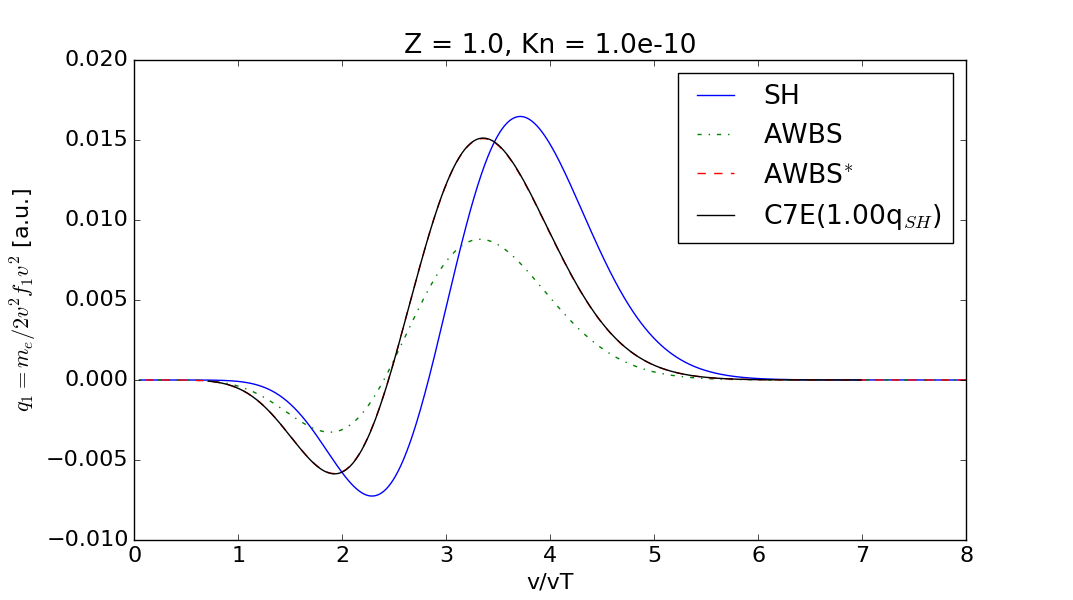
\includegraphics[width=0.7\textwidth]{../results/fe_analysis/diff_f1_comparison_Z1.png} \\
      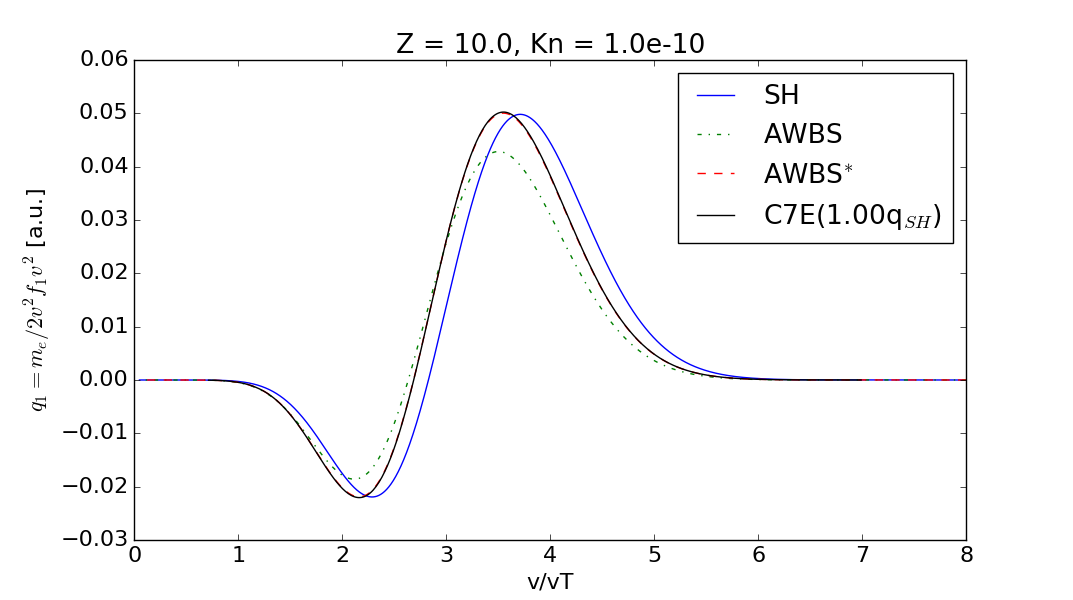
\includegraphics[width=0.7\textwidth]{../results/fe_analysis/diff_f1_comparison_Z10.png} \\
      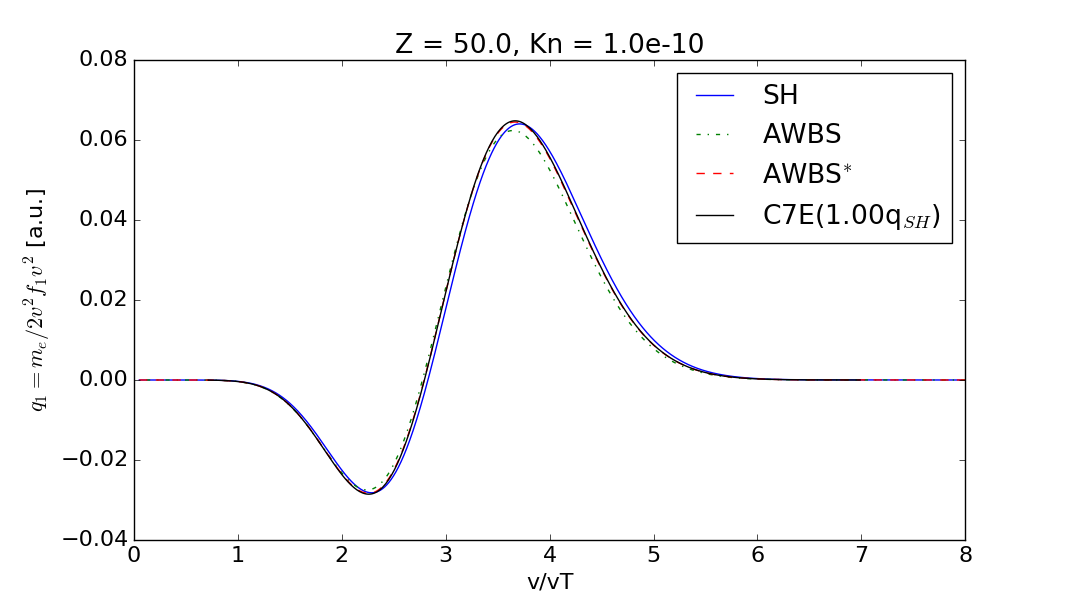
\includegraphics[width=0.7\textwidth]{../results/fe_analysis/diff_f1_comparison_Z50.png} 
    \end{tabular}
  \caption{
  The~diffusion asymptotic of AWBS with respect to SH using Z-correction 
  formula.
  }
  \end{center}
  \label{fig:AWBSvsSH_f1}
\end{figure}

\begin{figure}[tbh]
  \begin{center}
    \begin{tabular}{c}
      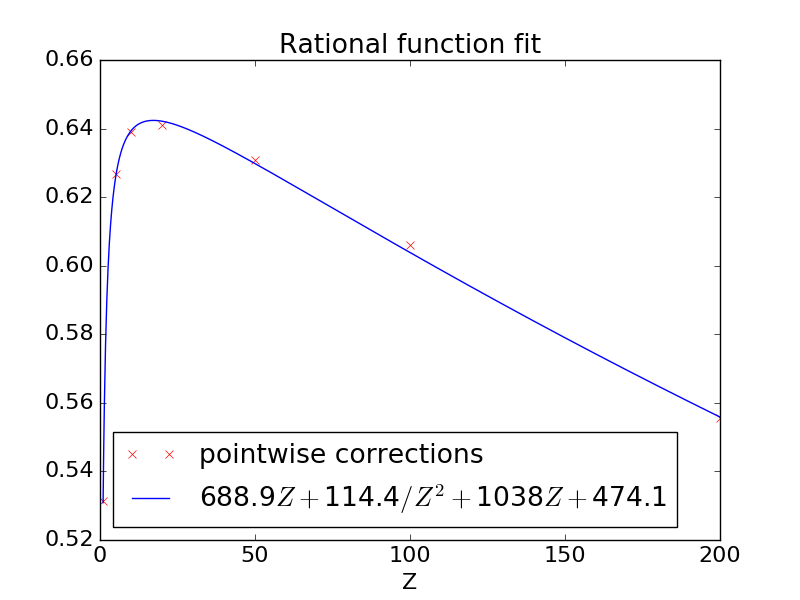
\includegraphics[width=0.8\textwidth]{../results/fe_analysis/diff_AWBScorrection_fit.png} 
    \end{tabular}
  \caption{
  Analytic fit to the~Z correction 
  ($\nu_{ei}^* = \frac{688.9 Z + 114.4}{Z^2 + 1038 Z + 474.1} \nu_{ei}$) 
  of the~diffusion asymptotic of AWBS with respect to SH.
  }
  \end{center}
  \label{fig:AWBScorrection_f1}
\end{figure}

\begin{figure}[tbh]
  \begin{center}
    \begin{tabular}{c}
      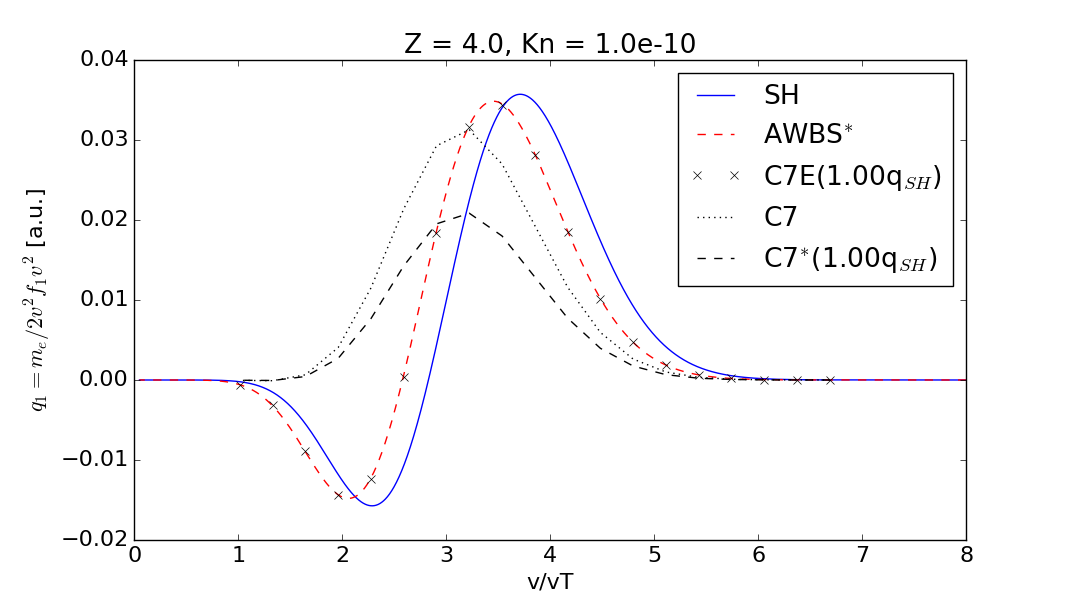
\includegraphics[width=0.8\textwidth]{../results/fe_analysis/diff_f1_C7AWBScorrection_Z4.png} 
    \end{tabular}
  \caption{
  Efficiency of C7 (18 groups). Definition of Efield free C7$^*$ calculation 
  based on reduction of the density of fast electrons.
  }
  \end{center}
  \label{fig:C7AWBScorrection}
\end{figure}

\begin{figure}[tbh]
  \begin{center}
    \begin{tabular}{cc}
      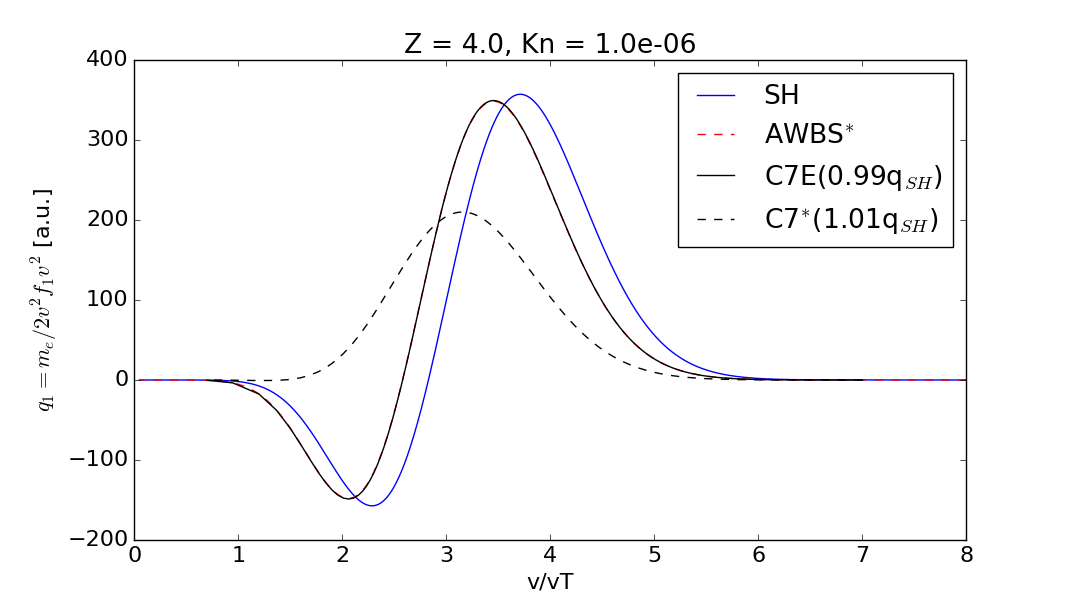
\includegraphics[width=0.5\textwidth]{../results/fe_analysis/f1_comparison_Kn1e-6_Z4.png} &
      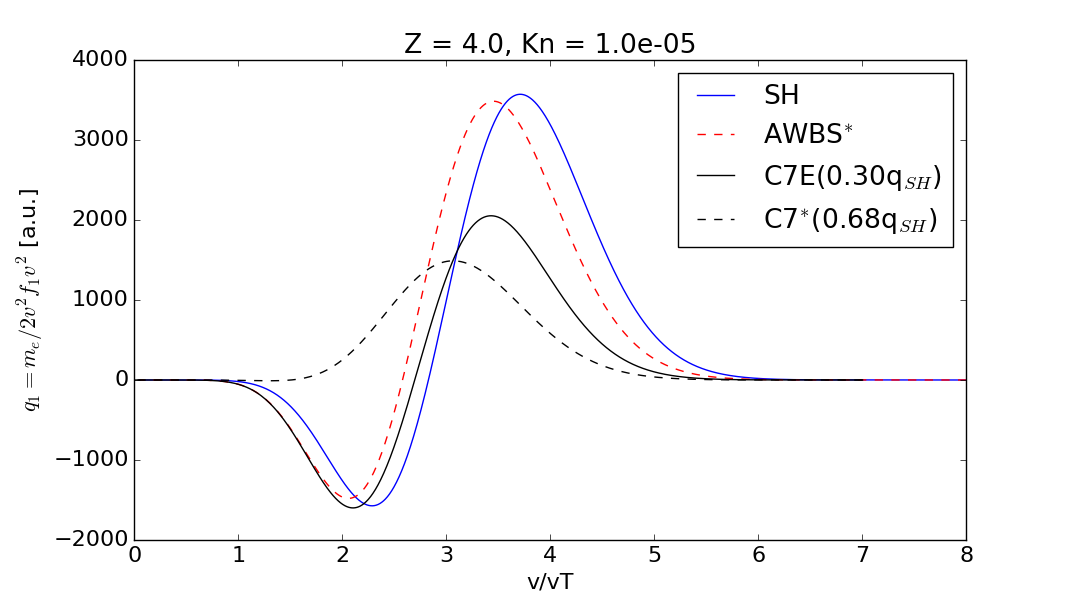
\includegraphics[width=0.5\textwidth]{../results/fe_analysis/f1_comparison_Kn1e-5_Z4.png} \\
       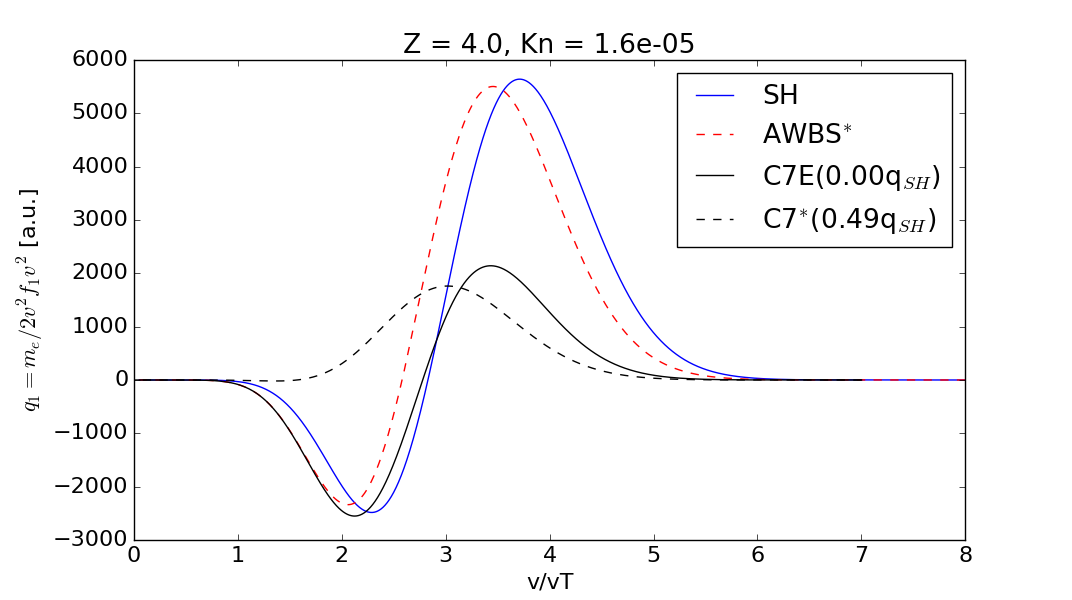
\includegraphics[width=0.5\textwidth]{../results/fe_analysis/f1_comparison_Kn16e-6_Z4.png} &
      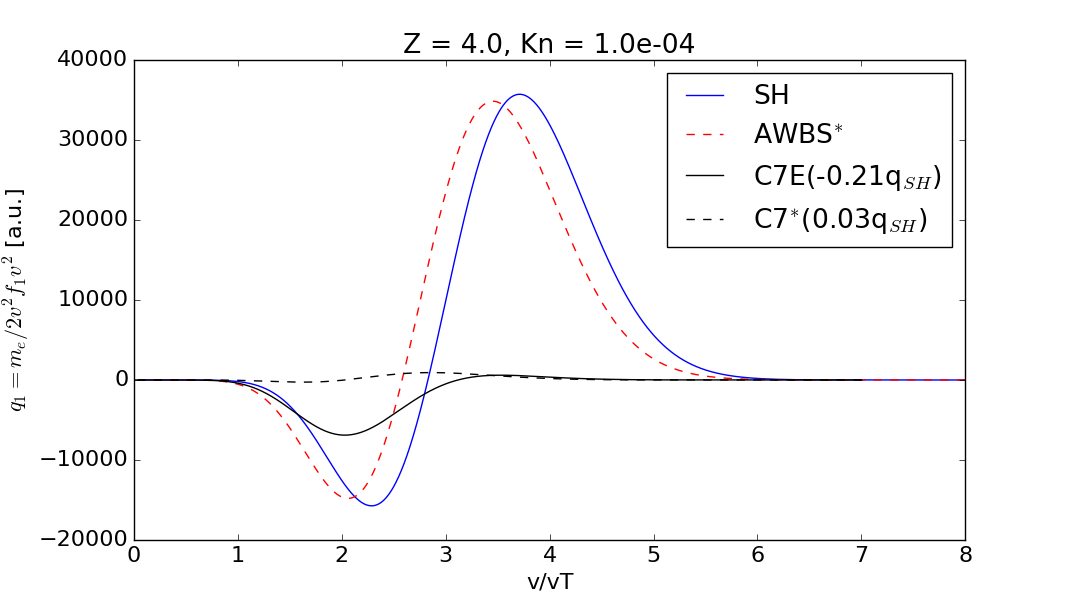
\includegraphics[width=0.5\textwidth]{../results/fe_analysis/f1_comparison_Kn1e-4_Z4.png}     
    \end{tabular}
  \caption{
  The~effect of the~diffusive electric field in AWBS model.
  }
  \end{center}
  \label{fig:EfieldAWBS}
\end{figure}

\clearpage

\section{Hydrodynamic diffusive electron collision operator HDECO}
\label{sec:diffusivecollisionoperator}
In order to improve the~electron collision operator AWBS analyzed 
in \secref{sec:AWBS_cop}, one can add the effect of diffusion in velocity space
as 
\begin{equation}
  \collpdv{f}{t} = \nue\vmag\pdv{}{\vmag}\left( f + 
  \frac{\vth^2}{\vmag} \pdv{f}{\vmag}\right) .
  \label{eq:DECO}
\end{equation}
Nevertheless, the~\textit{diffusive electron collision operator} \eqref{eq:DECO}
does not provide a~good bridge to hydrodynamics because of
\begin{equation}
  \collpdv{\fM - f}{t} = \collpdv{f}{t} ,
  \label{eq:DECOnobridge}
\end{equation}
i.e. there is no relation to hydrodynamics via temperature.
The~reason for \eqref{eq:DECOnobridge} is actually perfectly correct since
\begin{equation}
  \collpdv{\fM}{t} = 0 ,
  \qquad \implies\qquad \collpdv{f}{t} 
 \stackrel{ f\rightarrow\fM }{{\scalebox{3}[1]{=}}} 0,
  \label{eq:DECOfM}
\end{equation}
which directly demonstrates that \eqref{eq:DECOnobridge} obeys the~Boltzmann's
H-theorem. The~left side of (\ref{eq:DECOfM}) holds due to the~form of
Maxwell-Boltzmann distribution \eqref{eq:MBdistribution}.

A~non-trivial remedy of the~absence of bridge of the~electron distribution
function $f$ and the~background fluid modeled by hydrodynamics can be
found by introducing a~source of electrons, i.e. we propose 
the~"collision operator"
\begin{multline}
  \collpdv{f}{t} = n_i \ddv{\Zbar}{t}\frac{\fM(T)}{n_e} +
  \nue \vmag \pdv{}{\vmag}\left( f + 
  \frac{\vth^2}{\vmag} \pdv{f}{\vmag}\right) + \\
  \frac{\nuei}{2} 
  \left(\pdv{}{\mu}\left((1 - \mu^2)\pdv{f}{\mu}\right)
  + \frac{1}{\sin^2(\phi)}\frac{\partial^2f}{\partial\theta^2} \right) ,
  \label{eq:HDECO}
\end{multline}
where $\mu = \cos(\phi)$ and $n_i \ddv{\Zbar}{t}\frac{\fM(T)}{n_e}$ is a~source
of electrons, where the~distribution of ionized electrons is $\fM(T)$ 
(T corresponding to bounded "hydrodynamic" electrons).

Consequently, one can write the~simplified (linear) Boltzmann transport 
equation of electrons as
\begin{multline}
  \vn\cdot\nabla f + \frac{1}{\vmag} \left[ \tE\cdot\vn \pdv{f}{\vmag} 
  + \frac{\tE\cdot\vect{e}_\phi 
  - \vmag\tB\cdot\vect{e}_\theta}{\vmag}\pdv{f}{\phi}
  + \frac{\tE\cdot\vect{e}_\theta + \vmag\tB\cdot\vect{e}_\phi}
  {\vmag\sin(\phi)}\pdv{f}{\theta} \right] 
  =\\
  \frac{n_i}{\vmag}\ddv{\Zbar}{t}\frac{\fM(T)}{n_e} +
  \frac{\vmag}{\lambda^e}\pdv{}{\vmag}\left( f + 
  \frac{\vth^2}{\vmag} \pdv{f}{\vmag}\right) 
  + \frac{\fzero - f}{\lambda^{ei}} ,
  \label{eq:DECO_spherical}
\end{multline}
where $\mfpe$ is the~electron-electron mean free path, and
$\mfpei$ is the~electron-ion mean free path. We also approximate
$\mfpe = \Zbar \mfpei$. The~form of the~electron-ion scattering operator
arises form a~low anisotropy approximation 
($f\approx\fzero + \vn\cdot\fone$).

%% The Appendices part is started with the command \appendix;
%% appendix sections are then done as normal sections
%% \appendix

%% \section{}
%% \label{}

%% References
%%
%% Following citation commands can be used in the body text:
%% Usage of \cite is as follows:
%%   \cite{key}         ==>>  [#]
%%   \cite[chap. 2]{key} ==>> [#, chap. 2]
%%

%% References with bibTeX database:

\bibliographystyle{elsarticle-num}
\bibliography{NTH}

%% Authors are advised to submit their bibtex database files. They are
%% requested to list a bibtex style file in the manuscript if they do
%% not want to use elsarticle-num.bst.

%% References without bibTeX database:

% \begin{thebibliography}{00}

%% \bibitem must have the following form:
%%   \bibitem{key}...
%%

% \bibitem{}

% \end{thebibliography}


\end{document}

%%
%% End of file 
